\documentclass[aspectratio=169,11pt]{beamer}
% ==========================================================================
%  KSA lecture-slide theme  =  stock beamer "Boadilla"  +  KSA colour theme
%  brand colours sampled from the official KSA symbol mark:
%    Deep Prussian Blue  #2E3192   (지성 - intellect)
%    Golden Gray         #D6CBB1   (감성 - sensibility)
%  Engine: XeLaTeX.  Usage:
%    \documentclass[aspectratio=169,11pt]{beamer}
%    % ==========================================================================
%  KSA lecture-slide theme  =  stock beamer "Boadilla"  +  KSA colour theme
%  brand colours sampled from the official KSA symbol mark:
%    Deep Prussian Blue  #2E3192   (지성 - intellect)
%    Golden Gray         #D6CBB1   (감성 - sensibility)
%  Engine: XeLaTeX.  Usage:
%    \documentclass[aspectratio=169,11pt]{beamer}
%    % ==========================================================================
%  KSA lecture-slide theme  =  stock beamer "Boadilla"  +  KSA colour theme
%  brand colours sampled from the official KSA symbol mark:
%    Deep Prussian Blue  #2E3192   (지성 - intellect)
%    Golden Gray         #D6CBB1   (감성 - sensibility)
%  Engine: XeLaTeX.  Usage:
%    \documentclass[aspectratio=169,11pt]{beamer}
%    \input{../theme/ksa-theme.tex}
% ==========================================================================

\usepackage{fontspec}
\usepackage{amsmath,amssymb}
\usepackage{graphicx}
\graphicspath{{figs/}{../figs/}}
\usepackage{booktabs}
\usepackage{listings}

% ---- fonts (no ctex/xeCJK on this box -> fontspec drives CJK directly) -----
\defaultfontfeatures{Ligatures=TeX}
\setmainfont{Noto Sans CJK KR}
\setsansfont{Noto Sans CJK KR}
\setmonofont{Noto Sans Mono CJK KR}[Scale=0.92]

% ---- base theme: stock Boadilla ------------------------------------------
\usetheme{Boadilla}
\usefonttheme{professionalfonts}
\setbeamertemplate{navigation symbols}{}

% ---- KSA colour theme (recolour the stock theme) --------------------------
\definecolor{ksablue}{HTML}{2E3192}
\definecolor{ksabluedk}{HTML}{20226A}
\definecolor{ksagold}{HTML}{D6CBB1}
\definecolor{ksagolddk}{HTML}{A9976B}
\definecolor{ksared}{HTML}{C0392B}
\definecolor{ksagray}{HTML}{5B5B5B}

\setbeamercolor{structure}{fg=ksablue}
\setbeamercolor{alerted text}{fg=ksared}

\setbeamercolor{palette primary}{fg=white,           bg=ksablue}
\setbeamercolor{palette secondary}{fg=white,         bg=ksablue!85!black}
\setbeamercolor{palette tertiary}{fg=white,          bg=ksabluedk}
\setbeamercolor{titlelike}{fg=ksablue}
\setbeamercolor{frametitle}{fg=ksablue,bg=}
\setbeamercolor{title}{fg=ksablue}
\setbeamercolor{author}{fg=ksagray}
\setbeamercolor{institute}{fg=ksagray}
\setbeamercolor{block title}{fg=white,bg=ksablue}
\setbeamercolor{block body}{fg=black!85,bg=ksablue!6}
\setbeamercolor{item}{fg=ksablue}
\setbeamercolor{section in toc}{fg=black!85}

\setbeamerfont{frametitle}{series=\bfseries}
\setbeamerfont{title}{series=\bfseries}

% ---- footline:  KSA mark | "Made by ..." | n / N   (matches reference) ----
\newcommand{\ksacredit}{Made by Sumin Han \,\textperiodcentered\, suminhan@ksa.hs.kr}
\setbeamertemplate{footline}{%
  \hbox{%
    \begin{beamercolorbox}[wd=.18\paperwidth,ht=2.6ex,dp=1.5ex,leftskip=1.1em]{}%
      \raisebox{-0.35ex}{
\includegraphics[height=2.0ex]{ksa-logo.png}}%
    \end{beamercolorbox}%
    \begin{beamercolorbox}[wd=.64\paperwidth,ht=2.6ex,dp=1.5ex,center]{}%
      {\scriptsize\color{ksagray}\ksacredit}%
    \end{beamercolorbox}%
    \begin{beamercolorbox}[wd=.18\paperwidth,ht=2.6ex,dp=1.5ex,rightskip=1.1em]{}%
      \hfill{\scriptsize\color{ksablue}\insertframenumber\,/\,\inserttotalframenumber}%
    \end{beamercolorbox}%
  }%
  \vskip2pt
}

% ---- section divider: stock \sectionpage, KSA-coloured -------------------
\setbeamertemplate{section page}{%
  \begingroup\centering
    {\color{ksagolddk}\rule{0.16\paperwidth}{1pt}}\par\vskip1.0em
    {\usebeamerfont{title}\color{ksablue}\insertsectionhead\par}\vskip1.0em
    {\color{ksagolddk}\rule{0.16\paperwidth}{1pt}}\par
  \endgroup
}
\AtBeginSection[]{\begin{frame}[plain,noframenumbering]\vfill\sectionpage\vfill\end{frame}}

% ---- code listings ------------------------------------------------------------
\lstdefinestyle{ksa}{%
  basicstyle=\ttfamily\scriptsize,
  keywordstyle=\color{ksablue}\bfseries,
  commentstyle=\color{ksagray}\itshape,
  stringstyle=\color{ksagolddk},
  numberstyle=\tiny\color{ksagray},
  backgroundcolor=\color{ksablue!6},
  frame=leftline, framerule=1.4pt, rulecolor=\color{ksablue},
  xleftmargin=1em, aboveskip=0.8em, belowskip=0.4em,
  showstringspaces=false, breaklines=true, language=Python,
}
\lstset{style=ksa}

% ---- handy macros -----------------------------------------------------------
\newcommand{\kb}[1]{\textbf{\color{ksablue}#1}}   % blue keyword
\newcommand{\kq}[1]{\textbf{\color{ksared}#1}}    % red key-question

% ==========================================================================

\usepackage{fontspec}
\usepackage{amsmath,amssymb}
\usepackage{graphicx}
\graphicspath{{figs/}{../figs/}}
\usepackage{booktabs}
\usepackage{listings}

% ---- fonts (no ctex/xeCJK on this box -> fontspec drives CJK directly) -----
\defaultfontfeatures{Ligatures=TeX}
\setmainfont{Noto Sans CJK KR}
\setsansfont{Noto Sans CJK KR}
\setmonofont{Noto Sans Mono CJK KR}[Scale=0.92]

% ---- base theme: stock Boadilla ------------------------------------------
\usetheme{Boadilla}
\usefonttheme{professionalfonts}
\setbeamertemplate{navigation symbols}{}

% ---- KSA colour theme (recolour the stock theme) --------------------------
\definecolor{ksablue}{HTML}{2E3192}
\definecolor{ksabluedk}{HTML}{20226A}
\definecolor{ksagold}{HTML}{D6CBB1}
\definecolor{ksagolddk}{HTML}{A9976B}
\definecolor{ksared}{HTML}{C0392B}
\definecolor{ksagray}{HTML}{5B5B5B}

\setbeamercolor{structure}{fg=ksablue}
\setbeamercolor{alerted text}{fg=ksared}

\setbeamercolor{palette primary}{fg=white,           bg=ksablue}
\setbeamercolor{palette secondary}{fg=white,         bg=ksablue!85!black}
\setbeamercolor{palette tertiary}{fg=white,          bg=ksabluedk}
\setbeamercolor{titlelike}{fg=ksablue}
\setbeamercolor{frametitle}{fg=ksablue,bg=}
\setbeamercolor{title}{fg=ksablue}
\setbeamercolor{author}{fg=ksagray}
\setbeamercolor{institute}{fg=ksagray}
\setbeamercolor{block title}{fg=white,bg=ksablue}
\setbeamercolor{block body}{fg=black!85,bg=ksablue!6}
\setbeamercolor{item}{fg=ksablue}
\setbeamercolor{section in toc}{fg=black!85}

\setbeamerfont{frametitle}{series=\bfseries}
\setbeamerfont{title}{series=\bfseries}

% ---- footline:  KSA mark | "Made by ..." | n / N   (matches reference) ----
\newcommand{\ksacredit}{Made by Sumin Han \,\textperiodcentered\, suminhan@ksa.hs.kr}
\setbeamertemplate{footline}{%
  \hbox{%
    \begin{beamercolorbox}[wd=.18\paperwidth,ht=2.6ex,dp=1.5ex,leftskip=1.1em]{}%
      \raisebox{-0.35ex}{
\includegraphics[height=2.0ex]{ksa-logo.png}}%
    \end{beamercolorbox}%
    \begin{beamercolorbox}[wd=.64\paperwidth,ht=2.6ex,dp=1.5ex,center]{}%
      {\scriptsize\color{ksagray}\ksacredit}%
    \end{beamercolorbox}%
    \begin{beamercolorbox}[wd=.18\paperwidth,ht=2.6ex,dp=1.5ex,rightskip=1.1em]{}%
      \hfill{\scriptsize\color{ksablue}\insertframenumber\,/\,\inserttotalframenumber}%
    \end{beamercolorbox}%
  }%
  \vskip2pt
}

% ---- section divider: stock \sectionpage, KSA-coloured -------------------
\setbeamertemplate{section page}{%
  \begingroup\centering
    {\color{ksagolddk}\rule{0.16\paperwidth}{1pt}}\par\vskip1.0em
    {\usebeamerfont{title}\color{ksablue}\insertsectionhead\par}\vskip1.0em
    {\color{ksagolddk}\rule{0.16\paperwidth}{1pt}}\par
  \endgroup
}
\AtBeginSection[]{\begin{frame}[plain,noframenumbering]\vfill\sectionpage\vfill\end{frame}}

% ---- code listings ------------------------------------------------------------
\lstdefinestyle{ksa}{%
  basicstyle=\ttfamily\scriptsize,
  keywordstyle=\color{ksablue}\bfseries,
  commentstyle=\color{ksagray}\itshape,
  stringstyle=\color{ksagolddk},
  numberstyle=\tiny\color{ksagray},
  backgroundcolor=\color{ksablue!6},
  frame=leftline, framerule=1.4pt, rulecolor=\color{ksablue},
  xleftmargin=1em, aboveskip=0.8em, belowskip=0.4em,
  showstringspaces=false, breaklines=true, language=Python,
}
\lstset{style=ksa}

% ---- handy macros -----------------------------------------------------------
\newcommand{\kb}[1]{\textbf{\color{ksablue}#1}}   % blue keyword
\newcommand{\kq}[1]{\textbf{\color{ksared}#1}}    % red key-question

% ==========================================================================

\usepackage{fontspec}
\usepackage{amsmath,amssymb}
\usepackage{graphicx}
\graphicspath{{figs/}{../figs/}}
\usepackage{booktabs}
\usepackage{listings}

% ---- fonts (no ctex/xeCJK on this box -> fontspec drives CJK directly) -----
\defaultfontfeatures{Ligatures=TeX}
\setmainfont{Noto Sans CJK KR}
\setsansfont{Noto Sans CJK KR}
\setmonofont{Noto Sans Mono CJK KR}[Scale=0.92]

% ---- base theme: stock Boadilla ------------------------------------------
\usetheme{Boadilla}
\usefonttheme{professionalfonts}
\setbeamertemplate{navigation symbols}{}

% ---- KSA colour theme (recolour the stock theme) --------------------------
\definecolor{ksablue}{HTML}{2E3192}
\definecolor{ksabluedk}{HTML}{20226A}
\definecolor{ksagold}{HTML}{D6CBB1}
\definecolor{ksagolddk}{HTML}{A9976B}
\definecolor{ksared}{HTML}{C0392B}
\definecolor{ksagray}{HTML}{5B5B5B}

\setbeamercolor{structure}{fg=ksablue}
\setbeamercolor{alerted text}{fg=ksared}

\setbeamercolor{palette primary}{fg=white,           bg=ksablue}
\setbeamercolor{palette secondary}{fg=white,         bg=ksablue!85!black}
\setbeamercolor{palette tertiary}{fg=white,          bg=ksabluedk}
\setbeamercolor{titlelike}{fg=ksablue}
\setbeamercolor{frametitle}{fg=ksablue,bg=}
\setbeamercolor{title}{fg=ksablue}
\setbeamercolor{author}{fg=ksagray}
\setbeamercolor{institute}{fg=ksagray}
\setbeamercolor{block title}{fg=white,bg=ksablue}
\setbeamercolor{block body}{fg=black!85,bg=ksablue!6}
\setbeamercolor{item}{fg=ksablue}
\setbeamercolor{section in toc}{fg=black!85}

\setbeamerfont{frametitle}{series=\bfseries}
\setbeamerfont{title}{series=\bfseries}

% ---- footline:  KSA mark | "Made by ..." | n / N   (matches reference) ----
\newcommand{\ksacredit}{Made by Sumin Han \,\textperiodcentered\, suminhan@ksa.hs.kr}
\setbeamertemplate{footline}{%
  \hbox{%
    \begin{beamercolorbox}[wd=.18\paperwidth,ht=2.6ex,dp=1.5ex,leftskip=1.1em]{}%
      \raisebox{-0.35ex}{
\includegraphics[height=2.0ex]{ksa-logo.png}}%
    \end{beamercolorbox}%
    \begin{beamercolorbox}[wd=.64\paperwidth,ht=2.6ex,dp=1.5ex,center]{}%
      {\scriptsize\color{ksagray}\ksacredit}%
    \end{beamercolorbox}%
    \begin{beamercolorbox}[wd=.18\paperwidth,ht=2.6ex,dp=1.5ex,rightskip=1.1em]{}%
      \hfill{\scriptsize\color{ksablue}\insertframenumber\,/\,\inserttotalframenumber}%
    \end{beamercolorbox}%
  }%
  \vskip2pt
}

% ---- section divider: stock \sectionpage, KSA-coloured -------------------
\setbeamertemplate{section page}{%
  \begingroup\centering
    {\color{ksagolddk}\rule{0.16\paperwidth}{1pt}}\par\vskip1.0em
    {\usebeamerfont{title}\color{ksablue}\insertsectionhead\par}\vskip1.0em
    {\color{ksagolddk}\rule{0.16\paperwidth}{1pt}}\par
  \endgroup
}
\AtBeginSection[]{\begin{frame}[plain,noframenumbering]\vfill\sectionpage\vfill\end{frame}}

% ---- code listings ------------------------------------------------------------
\lstdefinestyle{ksa}{%
  basicstyle=\ttfamily\scriptsize,
  keywordstyle=\color{ksablue}\bfseries,
  commentstyle=\color{ksagray}\itshape,
  stringstyle=\color{ksagolddk},
  numberstyle=\tiny\color{ksagray},
  backgroundcolor=\color{ksablue!6},
  frame=leftline, framerule=1.4pt, rulecolor=\color{ksablue},
  xleftmargin=1em, aboveskip=0.8em, belowskip=0.4em,
  showstringspaces=false, breaklines=true, language=Python,
}
\lstset{style=ksa}

% ---- handy macros -----------------------------------------------------------
\newcommand{\kb}[1]{\textbf{\color{ksablue}#1}}   % blue keyword
\newcommand{\kq}[1]{\textbf{\color{ksared}#1}}    % red key-question


\title{정책기반 강화학습 (Policy-Based Reinforcement Learning)}
\subtitle{정책을 직접 파라미터화: 로그미분 트릭 \,$\cdot$\, REINFORCE와 CartPole \,$\cdot$\, 베이스라인/어드밴티지로 분산 줄이기}
\author{Machine Learning 2 \,\textperiodcentered\, 10주차}
\institute{한국과학영재학교 (KSA)}
\date{Chapter 10}

\begin{document}

% ===== title =====
\begin{frame}[plain,noframenumbering]
  \titlepage
\end{frame}

% ===== overview =====
\begin{frame}{이번 주차 개요}
  \begin{itemize}
    \item 로봇 팔의 관절에 가할 힘: $-10$Nm$\sim$$+10$Nm의 \kb{연속값} 중 아무거나.
    \item Ch.\,6$\cdot$9의 Q-learning/DQN은 매 스텝 $\max_{a'} Q(s',a')$ ---
      행동을 \textbf{나열해} 최댓값을 찾아야 함.
    \item 행동이 연속이면 후보가 \textbf{무한} --- argmax 자체가 불가능.
    \item 답: 행동 확률분포 $\pi_\theta(a|s)$를 신경망으로 표현해
      \textbf{정책을 직접 학습}. 최댓값을 ``찾는'' 대신 \textbf{샘플링}.
  \end{itemize}
  \vskip0.4em
  \begin{block}{세 차시의 흐름}
    \textbf{10.1} 정리를 세운다 --- softmax/조건부 정규 정책,
    로그미분 트릭 $\to$ Policy Gradient Theorem, 엔트로피 보너스, 분산 문제 \\
    \textbf{10.2} 정리를 알고리즘으로 --- REINFORCE 손계산, 2행동 밴딧,
    PyTorch CartPole, ``리턴을 그대로 쓰는'' 함정 \\
    \textbf{10.3} 거침을 고친다 --- 베이스라인/어드밴티지로 분산 감소,
    Actor-Critic, REINFORCE vs A2C 비교
  \end{block}
  \vskip0.3em
  {\footnotesize 이번 장의 REINFORCE/Actor-Critic 기초 위에 Ch.\,11에서
  PPO를 세우고, Ch.\,13--14의 로봇 시뮬레이션(Pendulum)이 그 위에 올라간다.
  심화 자료: Stanford CS234 (Reinforcement Learning).}
\end{frame}

% ================= SESSION 10.1 =================
\section{10.1 정책 그래디언트 정리}

\begin{frame}{두 경로: 가치기반 vs 정책기반}
  \begin{columns}[T]
    \begin{column}{0.58\textwidth}
      \begin{itemize}
        \item \textbf{좌측} 가치기반 (Ch.\,6$\cdot$9): 상태 $s_t$ $\to$
          Q-네트워크 $\to$ 각 행동의 가치 $Q(s,a)$ $\to$
          \textbf{argmax}로 행동 결정.
        \item \textbf{우측} 정책기반 (이번 장): $s_t$ $\to$ 정책 네트워크
          $\to$ 확률분포 $\pi_\theta(a|s_t)$ $\to$
          \textbf{샘플링}해 환경에 행동 전송.
        \item 환경은 두 경로 모두에 $r_{t+1}, s_{t+1}$ 반환.
        \item 우측: 리턴 $G_t$가 \textbf{곱수로} 그래디언트를 만들어
          policy update(경사 상승).
      \end{itemize}
    \end{column}
    \begin{column}{0.42\textwidth}
      \centering
      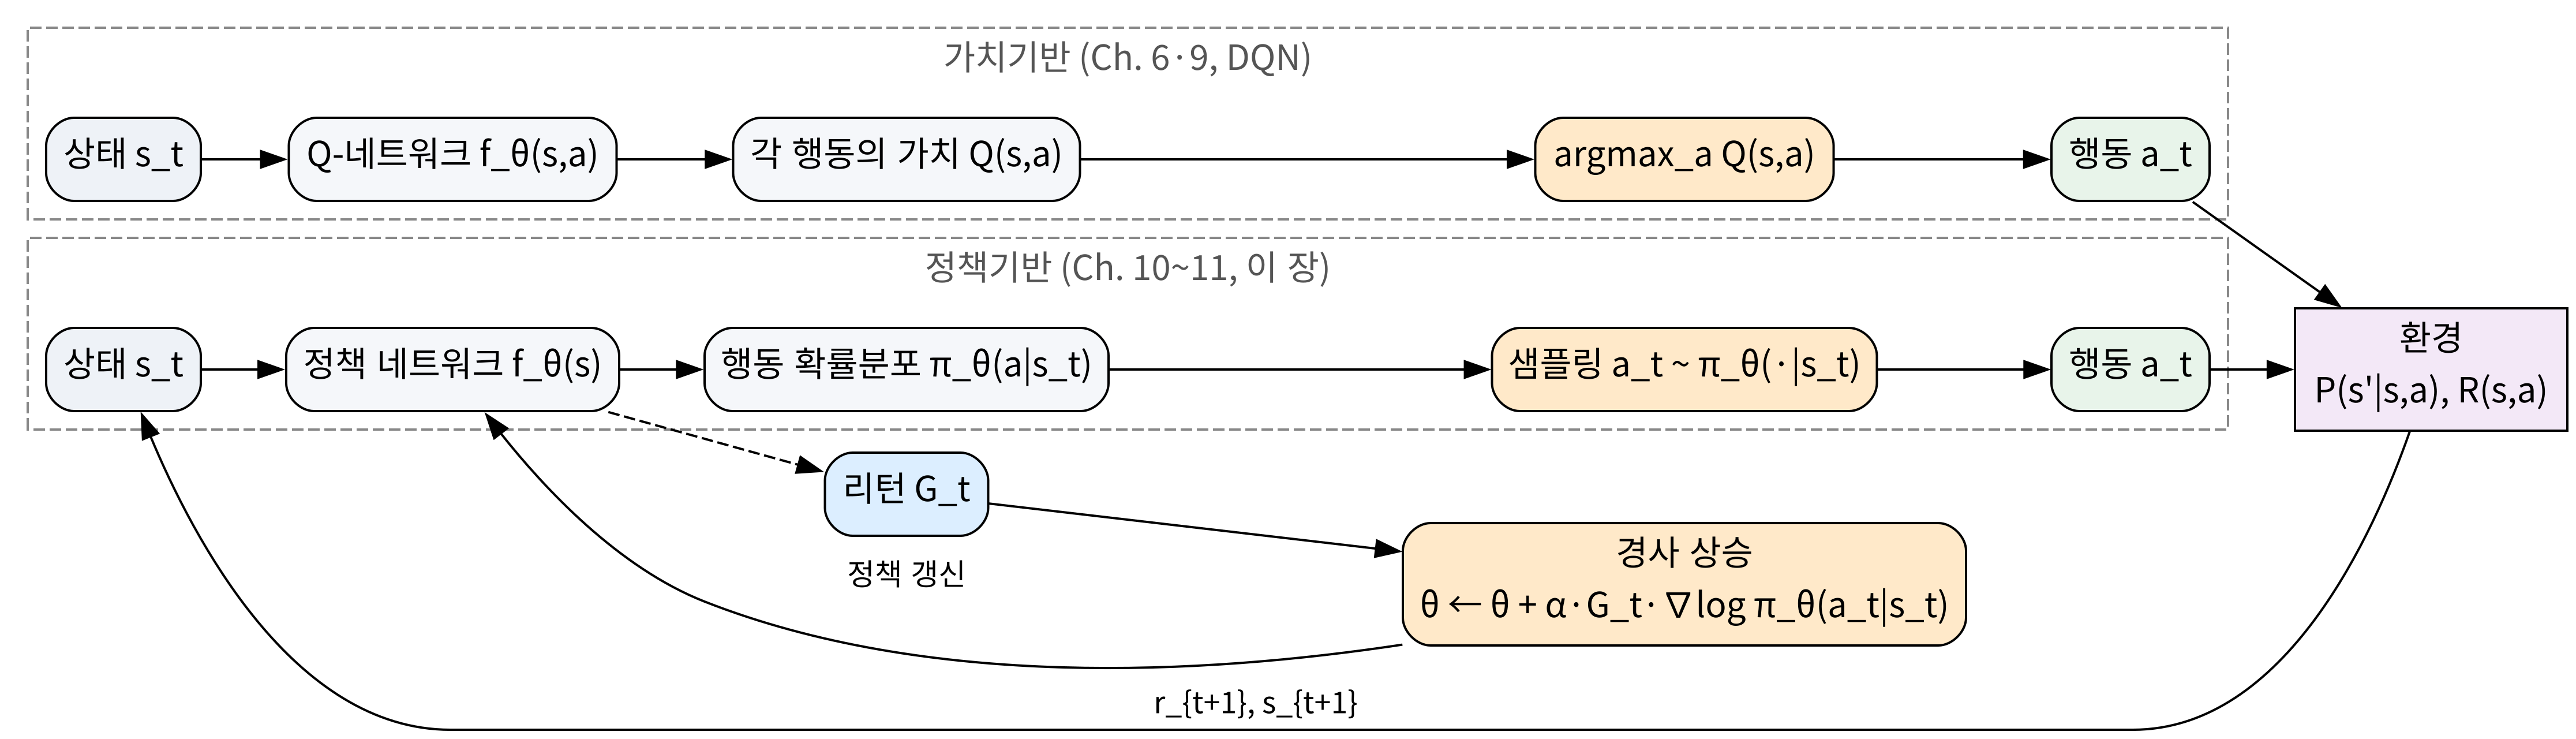
\includegraphics[width=\linewidth]{ch10_1_policy_based_flow.png}
      \vskip0.4em
      {\footnotesize 좌: 점수 내고 \textbf{최댓값} 뽑기.
      우: 확률 내고 \textbf{샘플링}.}
    \end{column}
  \end{columns}
  \vskip0.4em
  \kq{핵심 질문: ``점수를 올리는 방향''이 아니라
  \textbf{분포 자체를} 어떻게 고치겠는가?}
  --- Policy Gradient Theorem이 답하는 질문.
\end{frame}

\begin{frame}{``점수 $\to$ argmax'' 중간 단계를 건너뛴다}
  \begin{itemize}
    \item Ch.\,6$\cdot$9: $Q(s,a)$를 먼저 배우고,
      $\pi(s)=\arg\max_a Q(s,a)$ 로 \textbf{간접}적으로 정책 획득.
    \item \kb{정책기반 방법}: 이 중간 단계를 \textbf{건너뛰고},
      $\pi_\theta(a|s)$ (행동의 확률분포를 직접 내놓는 함수) 자체를
      신경망으로 표현해 학습.
    \item 연속 공간에서도 ``이 행동의 확률밀도가 얼마인가''는 잘
      정의됨 $\to$ argmax 문제가 자연스럽게 해결.
  \end{itemize}
  \vskip0.3em
  \begin{block}{이 선택의 대가, 한 줄로}
    가치기반 = \textbf{표}(각 행동의 ``얼마나 좋은지'')를 배우고 뒤에
    결정 규칙을 붙임. 정책기반 = 표를 버리고 \textbf{행동을 고르는 습관}을
    배우고 ``습관을 고치는 방향''을 보상으로 직접 계산.
    ``표 $\to$ 조회'' 두 단계가 ``샘플링'' 한 단계로 \textbf{병합}.
  \end{block}
  \vskip0.3em
  \begin{block}{용어: 이번 장의 ``정책''은 \kb{확률적(stochastic) 정책}}
    같은 상태에서 \textbf{여러 행동}을 각자 다른 확률로 고름 ---
    샘플링이 곧 탐험. (매 상태에서 항상 같은 행동인
    \textbf{결정적} $\pi(s)=a$ 는 Ch.\,6$\cdot$9의 argmax 방식이 본질적
    형태, Ch.\,13 DDPG/TD3/SAC에서 다룸.)
    ``정책 = 확률분포''로 읽으면 ``정책의 그래디언트''가
    $\nabla_\theta \log\pi_\theta(a|s)$, 즉 \textbf{확률의 미분}임이
    자연스럽게 읽힘.
  \end{block}
\end{frame}

\begin{frame}{이산 정책: softmax와 그 두 성질}
  \[
  \pi_\theta(a|s) = \text{softmax}(f_\theta(s))_a,
  \qquad
  p_a = \pi_\theta(a|s) = \frac{e^{z_a}}{\sum_{a'} e^{z_{a'}}}
  \]
  \begin{itemize}
    \item $f_\theta(s)$: 상태 $\to$ 각 행동의 \textbf{원점수(logit)}
      를 내는 신경망. softmax가 ``숫자''를 ``합이 1인 확률''로 변환.
    \item 목표: \kb{$J(\theta) = \mathbb{E}_{\tau \sim \pi_\theta}[R(\tau)]$}
      를 최대화. $\tau$ = 궤적(에피소드 전체), $R(\tau)$ = 총 보상.
  \end{itemize}
  \vskip0.3em
  \begin{block}{두 성질 --- 이번 절 전체에서 반복 등장}
    \textbf{(1) 합이 1} --- 한 행동의 확률을 올리면 \textbf{나머지는
    반드시 내려감} $\to$ one-vs-rest 그래디언트 모양의 이유.
    \textbf{(2) 미분 가능} --- $\theta$가 $z$를, $z$가 확률을
    \textbf{매끄럽게} 끔.
    \vskip0.2em
    ``미분 가능한 함수로 표현된 것''이 곧 \kb{파라미터화} =
    그래디언트 최적화의 \textbf{필요조건}.
  \end{block}
\end{frame}

\begin{frame}{연속 정책: 확률분포를 ``생성''하는 상태 조건부 정규}
  이산: 행동 유한 $\to$ softmax로 나열하면 끝. 연속 ($\mathbb{R}^d$:
  로봇 관절 각도, 힘의 크기): \textbf{확률밀도를 내는 분포 자체}가
  파라미터화 대상. 표준 선택:
  \[
  \pi_\theta(a|s) = \mathcal{N}\big(a\,;\, \mu_\theta(s),\; \Sigma_\theta(s)\big),
  \qquad
  a \sim \mathcal{N}\big(\mu_\theta(s),\, \Sigma_\theta(s)\big)
  \]
  \begin{itemize}
    \item 신경망 출력을 둘로 나눔: \textbf{평균} $\mu_\theta(s)$
      (``이 상태의 중심 행동'') $\cdot$ \textbf{분산} $\Sigma_\theta(s)$
      (``주변으로 얼마나 넓게 탐색'').
    \item $\Sigma$ 학습 $\to$ 탐색 강도가 \textbf{상태에 따라 달라지는}
      양 $\to$ 탐색-착취가 $\epsilon$-greedy(Ch.\,2) 같은 전역 상수가
      아니라 \textbf{상태별로 학습}. (Ch.\,13--14 Pendulum이 바로 이 구조)
    \item 흔한 변형: 표준편차 $\sigma_\theta(s)$를 \textbf{로그 스케일}로
      내서 $\Sigma = \text{diag}(\sigma_\theta^2)$.
      (대각 분산 = 각 관절 독립 탐색 = PPO 기본 설정)
  \end{itemize}
  {\footnotesize 로그밀도도 준비 --- 그래디언트 식의 $\log\pi$ 자리에:
  $\log\pi_\theta(a|s) = -\tfrac12(a-\mu_\theta)^T \Sigma_\theta^{-1}
  (a-\mu_\theta) - \tfrac12\log|\Sigma_\theta| - \tfrac{d}{2}\log 2\pi$}
\end{frame}

\begin{frame}{왜 정규분포인가 --- 세 가지 이유가 겹침}
  \begin{enumerate}
    \item \kb{지지가 전체} $\mathbb{R}^d$ --- 어떤 연속 행동도
      이론적으로 가능한 확률을 가짐.
    \item \kb{미분이 깨끗하다} --- 평균에 대해선
      $\nabla_\mu \log\pi = \Sigma^{-1}(a-\mu)$ 로 \textbf{선형},
      자유도 $d(d+1)/2$ 개.
    \item \kb{최대 엔트로피 원리} --- 이산의 softmax가 합 1 제약하의
      ``최대 엔트로피 분포''라면, 연속에서는 같은 원리가
      \textbf{정규분포}를 만듦. (아래 FAQ에서 증명)
  \end{enumerate}
  \vskip0.5em
  \begin{block}{한 줄}
    세 이유가 겹치므로 ``연속 정책의 표준 파라미터화 = 조건부 정규분포''.
  \end{block}
\end{frame}

\begin{frame}{엔트로피 보너스: 탐색이 ``학습 목표로'' 들어가도 되는가}
  \begin{itemize}
    \item softmax 이산 정책: 탐색은 \textbf{내장}(모든 로짓에서 모든
      행동에 양의 확률). 그런데 훈련하다 $\pi_\theta$ 가
      \textbf{디랙 근사}(한 행동만)로 수렴하면 탐색 \textbf{사라짐}.
    \item 표준 기법 = \kb{엔트로피 보너스}: 목적함수에 엔트로피를 더함.
  \end{itemize}
  \[
  J_{\text{ent}}(\theta) = \mathbb{E}_\tau[R(\tau)] - \beta\,
  \mathbb{E}_{s \sim \rho}\big[ H_\theta(s) \big],
  \quad
  H_\theta(s) := -\sum_a \pi_\theta(a|s)\log\pi_\theta(a|s)
  \]
  \begin{itemize}
    \item $H_\theta(s)$: 행동 분포가 얼마나 ``퍼져 있는가''.
      $H>0$ 유지 $\to$ 한쪽 확률 1로 수렴하는 퇴화 방지.
    \item $\beta=0$: 순수 리턴 최대화. $\beta$ 큼 $\to$ 탐색 강화.
      \textbf{$\beta$ 는 작게}(예: $10^{-3}$) --- 커지면 ``탐색만 하고
      보상엔 관심 없음''.
  \end{itemize}
  \vskip0.2em
  {\footnotesize 엔트로피의 그래디언트도 같은 구조:
  $\nabla_\theta \mathbb{E}_s[H_\theta] =
  \mathbb{E}_s[\mathbb{E}_{a\sim\pi}[\nabla_\theta\log\pi \,
  (-\log\pi_\theta(a|s))]]$ --- $\nabla_\theta\log\pi$ 로 표현.
  REINFORCE$\cdot$A2C$\cdot$PPO는 모두 $G_t$ 대신 $-\log\pi$ 를
  ``가중치''로 쓰는 \textbf{같은} 업데이트 식.
  (PPO 목적함수에도 $\mathbb{E}[\min(r_t \hat A_t, \text{clip}(\cdots))]
  - \beta H$ 로 포함)}
\end{frame}

\begin{frame}{``보상을 미분한다''와 벽의 두 얼굴}
  \begin{itemize}
    \item ``기대 보상을 최대화하는 $\theta$''를 \textbf{그대로}
      미분하려 하면: 기대 보상은 \textbf{무작위로} 행동해 얻은
      결과의 평균인데, 그 무작위성 자체가 $\theta$ 에 의존.
    \item 2행동 밴딧(보상 $+1/-1$, 1스텝, $s=1$ 고정)으로 펼쳐보면:
      \[
      J(\theta) = p_0(+1) + p_1(-1) = 2\,p_0(\theta) - 1
      \]
      --- $\theta$ 에 대해 \textbf{매끄럽게} 미분 가능, 벽은 아직 안 보임.
  \end{itemize}
  \vskip0.3em
  \begin{block}{벽은 두 얼굴로 분리된다}
    \textbf{(1) 적분의 미분} --- $\nabla_\theta$ 를 $\mathbb{E}$ 안으로
    넘기려면 분포가 $\theta$ 에 대해 미분 가능해야 함. 이산+유한이면
    유한 합으로 안전하나, \textbf{행동 연속이거나 상태 고차원}이면
    궤적 확률이 \textbf{적분} $\to$ 그 미분은 실제로 불가능.
    \vskip0.2em
    \textbf{(2) 단절된 샘플} --- 단일 샘플 추정치
    $\hat J = R(\tau_{\text{sample}})$ 는 $\theta$ 에 \textbf{무관한
    상수}(뽑힌 궤적은 이미 결정된 일) $\to$ 단일 추정치의 미분은 0.
    \vskip0.2em
    둘 다 \textbf{같은 ``분포의 미분'' 문제} --- 로그미분 트릭이
    \textbf{동시에} 해결.
  \end{block}
\end{frame}

\begin{frame}{로그미분 트릭과 Policy Gradient Theorem}
  \kb{로그미분 트릭} --- 항등식
  $\nabla_\theta \pi_\theta = \pi_\theta \nabla_\theta \log\pi_\theta$
  ($\nabla\log f = \nabla f/f$ 에서, $f>0$ 이면 무조건 성립):
  미분이 확률 \textbf{밖으로} 빠져나오지 않고, 다시 \textbf{기댓값
  형태}로 정리 가능. 최종 결과 --- \kb{Policy Gradient Theorem}
  (Williams, 1992; Sutton et al., 1999):
  \[
  \boxed{\; \nabla_\theta J(\theta)
  = \mathbb{E}_\tau\left[ \sum_t \nabla_\theta \log\pi_\theta(a_t|s_t)\; G_t
  \right] \;}
  \]
  \begin{itemize}
    \item $G_t$: 시점 $t$ 부터의 할인된 누적 보상 (Ch.\,3 return).
  \end{itemize}
  \kq{직관: ``결과가 좋았던($G_t$ 큰) 궤적에서 실제로 고른 행동의
  확률을 올리고, 나빴던 행동의 확률은 낮추는'' 방향으로 $\theta$ 이동.}
  \vskip0.3em
  {\footnotesize 왜 로그인가: $\nabla\pi$ 는 \textbf{절대} 변화율
  ($p$: 0.01$\to$0.02 와 0.9$\to$0.99 를 $+0.01$ 로 동률),
  $\nabla\log\pi = \nabla\pi/\pi$ 는 \textbf{상대} 변화율
  (``배율로 올린다''는 표현에 자연스러움). 상대 변화율이 기댓값 안의
  가중치가 되므로, ``기울어 있는 정도''를 샘플 하나로 추정 가능 ---
  ``단절된 단일 샘플'' 문제를 푸는 핵심 메커니즘.}
\end{frame}

\begin{frame}{유도: 궤적 확률에서 ``환경이 사라지는 순간''}
  \small
  궤적 $\tau=(s_0,a_0,r_1,s_1,\dots)$ 의 확률 = 환경 전이확률 $\times$
  정책:
  \[
  P(\tau;\theta) = P(s_0)\prod_t \pi_\theta(a_t|s_t)\; P(s_{t+1}|s_t, a_t)
  \]
  미분(유한 궤적 공간에서 합/미분 교환은 안전):
  \[
  \nabla_\theta J
  = \sum_\tau R(\tau)\, \nabla_\theta P(\tau;\theta)
  \]
  로그미분 트릭 적용 $\to$ 다시 기댓값 형태:
  \[
  \nabla_\theta P = P\, \nabla_\theta \log P
  \quad\Rightarrow\quad
  \nabla_\theta J = \mathbb{E}_\tau\big[ R(\tau)\,
  \nabla_\theta \log P(\tau;\theta) \big]
  \]
  \textbf{핵심 단계} --- $\log$ 로 곱을 합으로 분해:
  \[
  \log P(\tau;\theta) = \log P(s_0) + \sum_t
  \big[ \log\pi_\theta(a_t|s_t) + \log P(s_{t+1}|s_t, a_t) \big]
  \]
  $\theta$ 로 미분하면 $\log P(s_0)$ (상수)와
  $\log P(s_{t+1}|s_t,a_t)$ (환경, $\theta$ 와 무관)은
  \textbf{미분되자마자 0}:
  \[
  \nabla_\theta \log P(\tau;\theta) = \sum_t \nabla_\theta
  \log\pi_\theta(a_t|s_t)
  \]
  \normalsize
  {\footnotesize 무한 궤적 공간에서는 미분/적분 교환 조건 필요 ---
  정책 파라미터화가 매끄럽고 궤적 공간의 \textbf{측도가 $\theta$ 에
  무관}할 때 성립. 이 무관성이 model-free의 핵심.}
\end{frame}

\begin{frame}{최종 정리: $R$ 을 시점별 리턴 $G_t$ 로, 그리고 model-free}
  기댓값에 대입한 뒤, $R(\tau)=\sum_t r_t$ 를 시점별 \textbf{리턴}
  $G_t = \sum_{t'\ge t}\gamma^{t'-t} r_{t'}$ 로 바꿈:
  \[
  \nabla_\theta J(\theta)
  = \mathbb{E}_\tau\left[ \sum_t \nabla_\theta \log\pi_\theta(a_t|s_t)\; G_t
  \right],
  \qquad
  \hat g(\tau) = \sum_t \nabla_\theta \log\pi_\theta(a_t|s_t)\; G_t
  \]
  \begin{itemize}
    \item 각 $\nabla_\theta\log\pi(a_t|s_t)$ 가 \textbf{자기 시점부터의}
      $G_t$ 를 가중치로 씀 --- ``시점 $t$ 의 행동은 $t$ 이후의 보상만
      책임진다''는 \textbf{인과적 구조}.
    \item \textbf{단일 샘플 추정치} $\hat g(\tau)$ 의 \textbf{기댓값}이
      참 그래디언트 --- ``단절된 $R$'' 대신 \textbf{미분 가능한}
      $\nabla_\theta\log P$ 를 가중치로 쓴 셈.
      (10.2절 REINFORCE가 바로 이 $\hat g$ 를 계산)
  \end{itemize}
  \vskip0.3em
  \begin{block}{model-free의 핵심 성질이 ``사라진 항''에서 온다}
    $\nabla_\theta\log P(s_{t+1}|s_t,a_t) = 0$ 이라 최종 식에
    \textbf{환경 파라미터가 하나도} 남지 않음.
    $\Rightarrow$ \kb{환경 모델을 몰라도 정책을 학습할 수 있다} ---
    Ch.\,4 벨만방정식(환경 모델 전제)과 대비되는 정책기반의 본질.
  \end{block}
\end{frame}

\begin{frame}{``확률합 $=1$'' 제약이 만든 모양: one-vs-rest}
  2행동 softmax, $\theta=[\theta_0,\theta_1]$, 로짓 $z_k = \theta_k s$:
  \[
  \nabla_\theta \log\pi_\theta(0|s) = \big[(1-p_0)\,s,\; -p_1\,s\big],
  \qquad
  \nabla_\theta \log\pi_\theta(1|s) = \big[-p_0\,s,\; (1-p_1)\,s\big]
  \]
  \begin{itemize}
    \item \textbf{고른 행동}의 파라미터 성분 $(1-p_a)$,
      \textbf{고르지 않은} 행동 $-p_a$ --- \kb{one-vs-rest}.
    \item 유래 = ``확률합 $=1$'': $p_0 \uparrow$ 면 반드시
      $p_1 = 1-p_0$ 가 $\downarrow$.
    \item ``행동 0 확률 올리는 방향''은 구조적으로 ``행동 1 확률
      내리는 방향''과 \textbf{동일 벡터}.
  \end{itemize}
  \vskip0.3em
  {\footnotesize 이 제약이 만든 두 번째 성질은 다음 프레임 ---
  ``기대 그래디언트가 0''이라는, 10.2$\cdot$10.3 베이스라인 논리의
  공통 출발점.}
\end{frame}

\begin{frame}{수학적 핵심: $\mathbb{E}[\nabla_\theta\log\pi] = 0$}
  \[
  \mathbb{E}_{a \sim \pi(\cdot|s)}\big[\nabla_\theta \log\pi_\theta(a|s)\big]
  = \sum_a \pi_\theta(a|s)\, \nabla_\theta\log\pi_\theta(a|s)
  = \nabla_\theta \underbrace{\sum_a \pi_\theta(a|s)}_{= \,1}
  = 0
  \]
  세 단계:
  \begin{enumerate}
    \item $\nabla\log\pi = \nabla\pi/\pi$ 로 $\pi\nabla\log\pi = \nabla\pi$.
    \item 합과 미분의 교환.
    \item 확률합이 \textbf{상수 1}이므로 그 미분은 0.
  \end{enumerate}
  \vskip0.3em
  \begin{block}{숫자로 확인: $p_0=0.6,\, p_1=0.4$}
    \[
    0.6\,[0.4,\; -0.4] \;+\; 0.4\,[-0.6,\; 0.6]
    = [0.24, -0.24] + [-0.24, 0.24] = [0,\; 0]
    \]
    두 성분이 정확히 상쇄 --- 임의의 $\theta$ 에서 성립(우연 아님).
  \end{block}
  \vskip0.3em
  \kq{기억할 사슬: ``확률합 $=1$'' $\to$ ``기대 로그미분 그래디언트
  $=0$'' $\to$ \textbf{베이스라인 자유도}(10.2$\cdot$10.3의 논리가
  이 정리의 부수 결과로 읽힘).}
\end{frame}

\begin{frame}{정규 정책에도 같은 구조: 평균 갱신 = ``예측-실제 차이''}
  이산(softmax)이든 연속(정규)이든 $\nabla_\theta\log\pi$ 의
  \textbf{형태만} 바뀌고 Policy Gradient Theorem의 구조는 동일.
  정규 정책 $\pi_\theta(a|s) = \mathcal{N}(a;\, \mu_\theta(s),
  \sigma_\theta^2 I)$ (대각 분산, $\sigma$ 로그 스케일)에서:
  \[
  \nabla_{\mu} \log\pi_\theta(a|s)
  = \frac{(a - \mu_\theta(s))}{\sigma_\theta^2}
  \]
  \begin{itemize}
    \item ``실제로 고른 $a$ 가 예측 평균 $\mu$ 에서 얼마나 벗어나는가''를
      $\sigma^2$ 로 나눈 벡터.
    \item $a=\mu$ (예측 정확히 맞음) $\to$ 그래디언트 \textbf{0}
      --- ``고칠 것 없음''.
    \item $a > \mu$ 이고 $G_t>0$ $\to$ $\mu$ 를 \textbf{올리는} 방향
      --- ``예측보다 큰 행동을 골랐고 결과가 좋았으니, 예측 평균을
      그쪽으로''.
  \end{itemize}
  \vskip0.3em
  \begin{block}{이번 절에서 기억할 것}
    \textbf{평균 $\mu$ 의 갱신 = ``예측-실제 차이''의 방향}
    (분산 $\sigma^2$ 에 대한 그래디언트도 존재 --- 10.3 A2C/PPO에서
    $\sigma$ 동시 학습). 이 직관이 Ch.\,11 PPO ``왜 $\sigma$ 를
    클리핑하지 않는가'' 질문의 출발점.
  \end{block}
\end{frame}

\begin{frame}{손으로 한 스텝 (1/2): 좋은 경우 $G_t = +1$}
  2행동 밴딧(보상 $+1/-1$, 1스텝, $s=1$).
  $\theta=[1,0]$, $\alpha=0.1$, $G_t=+1$ (행동 0 샘플링).
  \[
  p_0 = \text{softmax}([1,0])_0 = \frac{e^1}{e^1+1} \approx 0.7311,
  \qquad p_1 \approx 0.2689
  \]
  \[
  \nabla_\theta \log\pi_\theta(0|1) = \big[(1-0.7311),\; -0.2689\big]
  = [0.2689,\; -0.2689]
  \]
  갱신(경사 상승 --- 최대화이므로 $+$):
  \[
  \theta \leftarrow [1,0] + 0.1 \times 1 \times [0.2689, -0.2689]
  = [1.0269,\; -0.0269]
  \]
  새 정책: $p_0' \approx \mathbf{0.7415}$, $p_1' \approx 0.2585$.
  \begin{block}{읽어볼 것}
    $p_0$: $0.7311 \to \mathbf{0.7415}$로 \textbf{올랐다} ---
    좋은 결과를 낸 행동 0의 확률이 실제로 증가.
    $p_1$ 도 $0.2689 \to 0.2585$로 \textbf{내려감} ---
    one-vs-rest의 ``고르지 않은 행동도 갱신된다'' 성질.
  \end{block}
\end{frame}

\begin{frame}{손으로 한 스텝 (2/2): 나쁜 경우 $G_t = -1$}
  같은 초기 $\theta=[1,0]$, 이번엔 $G_t=-1$, \textbf{행동 1} 샘플링:
  \[
  \nabla_\theta \log\pi_\theta(1|1) = \big[-0.7311,\; (1-0.2689)\big]
  = [-0.7311,\; 0.7311]
  \]
  \[
  \theta \leftarrow [1,0] + 0.1 \times (-1) \times [-0.7311,\; 0.7311]
  = [1.0731,\; -0.0731]
  \]
  새 정책: $p_0' \approx \mathbf{0.7588}$, $p_1' \approx 0.2412$.
  \begin{itemize}
    \item $G_t=-1$(나쁜 결과)가 행동 1에 부여 $\to$
      ``나쁜 결과를 낸 행동 1의 확률을 내리자''.
    \item $p_1$: $0.2689 \to 0.2412$로 내려가는 \textbf{대신},
      합 1 제약 때문에 $p_0$ 가 \textbf{자동으로} 올라감.
  \end{itemize}
  \vskip0.4em
  \kq{``나쁜 행동을 내리면 좋은 행동은 자동으로 올라간다''
  --- 이것이 one-vs-rest 구조의 \textbf{본질}.}
  {\footnotesize 10.2절 ``손으로 한 번 갱신하기'' 블록이 같은 계산
  ($\alpha=0.1$, $G=\pm 3$)을 더 크게 보여준다.}
\end{frame}

\begin{frame}{정리의 ``약점'': 기댓값은 정확하지만 분산이 크다}
  \begin{itemize}
    \item 기댓값은 정확하나, 단일 샘플 $\hat g(\tau)$ 의 분산이
      \textbf{크다} --- $G_t$ 가 \textbf{에피소드 전체} 보상 누적
      이라 \textbf{운}(초기 상태의 불운, 중간 선택의 불운)에 크게 의존.
    \item 같은 $\theta$ 로 두 에피소드: 행운으로 오래 버튼 쪽은
      $G_t$ 크게 양수, 불운으로 일찍 끝난 쪽은 작음(또는 음수).
      평균은 참 값에 가깝지만 \textbf{단일} 샘플은 멀리.
    \item \kb{몬테카를로 추정}이 바로 가능한 이유도 기대 형태:
      참 그래디언트 $\mathbb{E}_\tau[\cdot]$, 단일 샘플 $\hat g$,
      N 샘플 $\hat g_N = \frac1N \sum_i \hat g(\tau_i)$
      $\xrightarrow{N\to\infty}$ 참 그래디언트(대수법칙).
  \end{itemize}
  \vskip0.3em
  \begin{block}{10.2절에서 숫자로 확인될 것}
    REINFORCE CartPole 300 에피소드: 처음 20 에피소드 평균 14.1
    $\to$ 마지막 20 에피소드 평균 99.5. 시드 세 번을 바꾸면
    \textbf{곡선 모양이 다름} --- 어떤 시드는 194 에피소드만에
    250 돌파, 다른 시드는 300까지 150 안팎.
    \textbf{같은 알고리즘, 같은 환경, 다른 곡선}.
  \end{block}
\end{frame}

\begin{frame}{이산 vs 연속: 두 정책 파라미터화 한눈에}
  \scriptsize
  \begin{tabular}{@{}lll@{}}
    \toprule
     & 이산 (softmax) & 연속 (정규) \\
    \midrule
    행동 공간 & 유한 $\{0,1,\dots\}$ & $\mathbb{R}^d$ \\
    분포 & 카테고리컬 & 가우시안 $\mathcal{N}(\mu,\Sigma)$ \\
    신경망 출력 & 로짓 $z_a$ (각 행동 하나) & 평균 $\mu$ + 분산 $\Sigma$ \\
    로그밀도 & $\log z_a - \log\sum_{a'} z_{a'}$ &
      $-\tfrac12(a-\mu)^T\Sigma^{-1}(a-\mu)
      -\tfrac12\log|\Sigma| - \tfrac d2 \log 2\pi$ \\
    $\nabla_\theta \log\pi$ & one-vs-rest & $\Sigma^{-1}(a-\mu)$ (평균 부분) \\
    탐색 메커니즘 & softmax 자체 & 분산 $\Sigma$ 학습 \\
    엔트로피 & $-\sum_a p_a \log p_a$ & $\tfrac{d}{2}(1 + \log 2\pi e\, \sigma^2)$ \\
    사용 장소 & CartPole, Atari & 로봇 시뮬레이션 (Ch.\,13--14) \\
    \bottomrule
  \end{tabular}
  \normalsize
  \vskip0.5em
  \begin{block}{구조 동일성이 policy gradient의 힘}
    둘 다 $\nabla_\theta J = \mathbb{E}[\sum_t \nabla_\theta
    \log\pi_\theta(a_t|s_t)\,G_t]$ 를 공유 ---
    다만 $\nabla_\theta\log\pi$ 의 \textbf{형태만} 다름.
  \end{block}
  {\footnotesize 주의: 엔트로피 행 --- 이산(비트 단위)과 연속(자연로그
  단위)의 \textbf{단위가 다름} $\to$ $\beta$(엔트로피 보너스 계수)를
  이산$\leftrightarrow$연속 사이에 직접 이관 불가. Ch.\,13--14에서
  $\beta$ 튜닝 시 직접 부딪힘.}
\end{frame}

\begin{frame}{확인 문제 (10.1)}
  \small
  \begin{enumerate}
    \item \kb{벽의 두 얼굴} --- (a) 적분의 미분, (b) 단절된 샘플을
      로그미분 트릭이 각각 어떻게 해결하는지 한 문장씩.
      (힌트: ``미분이 확률 밖으로 나간다''의 구체적 의미)
    \item \kb{3단계 증명} --- $\mathbb{E}[\nabla_\theta\log\pi]=0$ 증명
      중 어느 단계가 실제로 ``제약 $\sum_a\pi=1$''을 쓰나?
      (힌트: 상수 $1$의 미분이 0인 사실은 제약 없이는 성립하지 않음)
    \item \kb{연속 정책} --- $\nabla_\mu\log\pi = (a-\mu)/\sigma^2$
      도출. $a=5,\ \mu=3,\ \sigma^2=1$ 에서 값 계산하고,
      $G_t=+2$ 일 때 $\mu$ 방향 예측.
    \item \kb{이산 vs 연속} --- 엔트로피 두 형태의 차이(단위: 비트 vs
      냅)와 그것이 $\beta$ 튜닝에 미치는 실무적 영향.
    \item \kb{model-free} --- ``환경이 사라지는 순간''이 없으면
      무엇이 깨지는가? (힌트: ``환경 모델을 몰라도 정책 학습'')
  \end{enumerate}
  \normalsize
\end{frame}

\begin{frame}{역사: ``스코어 함수'' 뒤에 숨은 100년}
  \begin{itemize}
    \item ``로그미분 트릭''이라는 \textbf{이름}은 RL 문헌에서
      1990년대에 정착, \textbf{수학}은 훨씬 오래됨.
    \item $\nabla\log f = \nabla f/f$ 는 미분 공부 첫 달의 기본 공식.
    \item 기댓값 내 미분을 샘플로 추정하는 기법은 통계학에서
      \kb{스코어 함수 추정치}(score function estimator)로
      1900년대 초부터 존재 --- 스코어 함수 $\nabla_\theta\log f(x;\theta)$
      는 \textbf{최대 우도 추정(MLE)}의 핵심(우도의 로그를 미분해
      0이 되는 점 찾기).
    \item Williams (1992)가 정책 그래디언트를 정식 논증할 때,
      동일 알고리즘을 스코어 함수 추정치와 \textbf{정확히 동일}하게
      식별 $\to$ ``RL 발명''이 아니라 \textbf{고전 통계 기법의
      RL 적용}.
  \end{itemize}
  \vskip0.3em
  {\footnotesize 반면 Sutton의 1984년 박사논문에는 이미 ``행동의
  결과를 보면서 행동 확률을 조정''하는 같은 계열 알고리즘이 있음
  --- \textbf{수학적 근거가 알고리즘 발명 이후에 정식화된} 예.
  ``발명 이후 이론화''가 policy gradient 방법의 특별한 역사.
  (10.2절 역사에서 다시 만남)}
\end{frame}

\begin{frame}{자주 하는 실수 (10.1)}
  \kb{1. $\nabla\log\pi$ 와 $\nabla\pi$ 혼용}
  \begin{itemize}
    \item 항등식 $\nabla_\theta\pi = \pi\,\nabla_\theta\log\pi$ 로
      \textbf{전환 가능}하나 \textbf{동일하지 않음}:
      절대 변화율 vs 상대 변화율.
    \item 실습에서 \texttt{log\_prob} 대신 \texttt{prob} 를 직접
      미분하면 \textbf{분산이 급격히 증가} --- $\pi$ 가 작은 행동에서
      $\nabla\pi$ 도 작아져 \textbf{신호가 희미}해짐.
  \end{itemize}
  \vskip0.4em
  \kb{2. 기댓값 내 미분 교환 조건 무시}
  \begin{itemize}
    \item $\nabla_\theta$ 와 $\mathbb{E}$ 교환이 안전하려면:
      정책 파라미터화 \textbf{매끄럽고}, 궤적 공간의 \textbf{측도가
      $\theta$ 에 무관}해야 함.
    \item 조건이 깨지면(예: $\theta$ 에 의존하는 가변 크기의 유한 합
      행동 공간) \textbf{정리 자체가 성립하지 않음}.
  \end{itemize}
  \vskip0.4em
  \kb{3. 베이스라인이 행동 $a$ 에 의존하는 값 사용}
  \begin{itemize}
    \item $b$ 가 $a$ 에 의존하면 $\mathbb{E}[\nabla_\theta\log\pi \cdot b]=0$
      이 \textbf{깨져 편향} 발생 (``한 적이 많으면 더 크게 빼자''의
      $b(a,s)$ 가 예).
    \item \textbf{베이스라인은 상태 $s$ 에만 의존해야 한다}.
  \end{itemize}
\end{frame}

\begin{frame}{FAQ: 정규분포는 왜 ``최대 엔트로피'' 분포인가}
  \begin{itemize}
    \item 이산: ``무차별 시 엔트로피 최대'' 원리 $\to$ 모든 행동에
      균등 확률 $1/K$ $\to$ 엔트로피 최대 분포 = \textbf{균등 분포}.
    \item 연속: \textbf{같은} 원리를 적용하면 \textbf{정규분포}.
  \end{itemize}
  \vskip0.3em
  \begin{block}{증명 (변분법, 간단)}
    엔트로피 $h(p)$ 를 $p$ 에 대해 최대화하되
    $\mathbb{E}_p[x] = \mu$, $\mathbb{E}_p[x^2] = \mu^2 + \sigma^2$
    제약 아래 변분하면, 결과 분포
    $p(x) = \exp(-\lambda_0 - \lambda_1 x - \lambda_2 x^2)$
    --- \textbf{정규분포}.
  \end{block}
  \vskip0.3em
  \begin{itemize}
    \item $\to$ 정규 정책이 ``\textbf{가장 보수적} 파라미터화'':
      평균$\cdot$분산 제약 아래 엔트로피 최대 = ``정보를 최소로
      가정''하는 분포. 학습 초기엔 \textbf{안전}하나, 복잡한 분포
      구조의 행동 공간에선 \textbf{표현력 한계}.
  \end{itemize}
  {\footnotesize 한계 극복 연구: GAN 기반 정책, 미분 가능
  정상 흐름 (normalizing flow) 정책.}
\end{frame}

\begin{frame}{자주 묻는 질문 (10.1)}
  \small
  \begin{itemize}
    \item \kb{Q: 정책기반이 가치기반보다 항상 나은가?}
      \textbf{아님.} 연속 공간에선 사실상 유일 선택지이나, 이산
      공간이 작고 데이터가 충분하면 Q-learning/DQN이 더 \textbf{안정적}
      이고 \textbf{데이터 효율적}인 경우가 많음 (10.2 실습에서
      CartPole로 직접 비교).
    \item \kb{Q: 연속 공간의 $\pi_\theta(a|s)$ 는 어떤 형태?}
      신경망이 정규분포의 $\mu_\theta(s),\sigma_\theta(s)$ 를 출력,
      행동은 그 분포에서 샘플링. 로그미분 트릭은 이산/연속
      \textbf{동일}($\log\pi$ 가 정규 로그밀도로 바뀔 뿐).
      Ch.\,13--14 로봇 시뮬레이션이 바로 이 구조.
    \item \kb{Q: 결정적 정책 $\pi(s)=a$ 에는?}
      이 정리는 \textbf{확률적} 정책에 대한 것. 결정적 정책은
      샘플링 단계가 없으므로 $\nabla_\theta\log\pi$ 대신
      $\nabla_\theta a$ 가 등장 (Ch.\,13 DDPG/TD3/SAC).
      둘 다 policy gradient family이나 \textbf{미분 대상이 다름}.
    \item \kb{Q: ``기댓값이 정확하다''의 정확한 의미?}
      $\mathbb{E}[\hat g(\tau)] = \nabla_\theta J$(참 그래디언트) ---
      단일 샘플 $\hat g(\tau)$ 자체가 참 값과 멀어질 수 있음(분산 큼).
      ``기댓값 정확'' $\ne$ ``단일 샘플 정확''.
  \end{itemize}
  \normalsize
\end{frame}



% ================= SESSION 10.2 =================
\section{10.2 REINFORCE와 실습}

\begin{frame}{위치: 정리에서 알고리즘으로}
  10.1에서 ``무작위 결과인데도 미분할 수 있다''는 큰 걸음 ---
  Policy Gradient Theorem:
  \[
  \nabla_\theta J(\theta) = \mathbb{E}_\tau\left[ \sum_t
  \nabla_\theta \log\pi_\theta(a_t|s_t)\, G_t \right]
  \]
  \begin{itemize}
    \item 그런데 ``식은 얻었다''와 ``실행할 수 있다''는 \textbf{다른 문제}.
    알고리즘으로 바꾸려면 두 질문을 답해야:
  \end{itemize}
  \begin{enumerate}
    \item \textbf{$\nabla_\theta\log\pi_\theta(a_t|s_t)$ 는 어떤
      \textbf{모양}인가?} --- softmax 파라미터화에 대해 실제로 미분.
    \item \textbf{$\mathbb{E}_\tau$ 는 어떤 \textbf{샘플}로 추정하나?}
      --- 가장 단순한 선택: 현재 정책으로 에피소드 \textbf{한 번}
      굴려서, 실제로 관찰한 $G_t$ 와 실제로 고른 행동의
      $\log\pi_\theta$ 를 사용.
  \end{enumerate}
  \vskip0.3em
  \begin{block}{이번 절의 \kb{REINFORCE}}
    이 ``가능한 가장 단순한'' 선택을 \textbf{모두} 채택한 알고리즘.
    이 \textbf{단순함} 그 자체가 교육적 가치 (``역사''에서 다시 볼
    것) --- 이동 부품을 최소화해서 \textbf{코드 한 줄이 정리 한 항과
    직접 대응}.
  \end{block}
\end{frame}

\begin{frame}[fragile]{REINFORCE: 정리를 그대로 경사 상승으로}
\begin{lstlisting}
import math

def softmax_policy(theta, state_feature):
    logits = [theta[0]*state_feature, theta[1]*state_feature]
    m = max(logits)
    exps = [math.exp(l - m) for l in logits]   # 수치 안정화
    total = sum(exps)
    return [e / total for e in exps]

def reinforce_update(theta, episode, alpha, gamma):
    # episode: [(state_feature, action, reward), ...]
    T = len(episode)
    G = [0.0] * T
    running = 0.0
    for t in reversed(range(T)):            # 루프 1: 리턴 G_t 역산
        running = episode[t][2] + gamma * running
        G[t] = running
    for t, (s, a, r) in enumerate(episode): # 루프 2: 스텝별 갱신
        probs = softmax_policy(theta, s)
        if a == 0:
            grad_log_pi = [(1 - probs[0]) * s, -probs[1] * s]
        else:
            grad_log_pi = [-probs[0] * s, (1 - probs[1]) * s]
        theta[0] += alpha * G[t] * grad_log_pi[0]
        theta[1] += alpha * G[t] * grad_log_pi[1]
    return theta
\end{lstlisting}
  \vskip0.2em
  {\footnotesize 정책은 \textbf{가능히 가장 단순한} 형태: 1차원 상태
  특징 $s$ 에 대한 \textbf{선형 로짓} $(\theta_0 s, \theta_1 s)$ 에
  softmax --- 신경망은 등장하지 않음. 실제(아래 PyTorch
  \texttt{PolicyNet})에서는 선형 부분을 $f_\theta(s)$ 신경망으로 바꿀
  뿐, \textbf{갱신 식의 구조는 동일}.}
\end{frame}

\begin{frame}{코드가 실제로 하는 일: 두 개의 루프와 one-vs-rest}
  \begin{columns}[T]
    \begin{column}{0.5\textwidth}
      \kb{루프 1 (뒤에서부터): 리턴 $G_t$ 계산}
      \begin{itemize}
        \item 마지막 스텝에서 시작해
          $G_t = r_t + \gamma G_{t+1}$ 로 \textbf{거꾸로 누적}.
        \item Ch.\,3의 리턴 정의, 그대로.
      \end{itemize}
    \end{column}
    \begin{column}{0.5\textwidth}
      \kb{루프 2 (앞에서부터): 스텝별 갱신}
      \begin{itemize}
        \item (a) 현재 $\pi_\theta$ 로 $p_0, p_1$ 계산.
        \item (b) 실제로 고른 $a_t$ 의
          $\log\pi_\theta(a_t|s_t)$ 그래디언트 계산.
        \item (c) 그걸 $G_t$ 로 \textbf{곱해} $\theta$ 조금
          옮김 ($+=$ --- 경사 \textbf{상승}).
      \end{itemize}
    \end{column}
  \end{columns}
  \vskip0.4em
  \begin{block}{softmax 그래디언트의 모양 --- one-vs-rest}
    \[
    \frac{\partial \log\pi_\theta(0|s)}{\partial\theta}
    = \big[(1-p_0)s,\; -p_1 s\big],
    \qquad
    \frac{\partial \log\pi_\theta(1|s)}{\partial\theta}
    = \big[-p_0 s,\; (1-p_1)s\big]
    \]
    고른 행동 $(1-p_a)$, 나머지는 $-p_a$. 이유 = \textbf{확률합
    항상 1} --- 한 확률을 올리면 다른 것이 \textbf{반드시} 내려가므로,
    ``고른 행동을 올리는'' 갱신은 ``고르지 않은 것을 내리는''
    갱신이 \textbf{동시에} 됨.
  \end{block}
  {\footnotesize 두 루프 순서가 REINFORCE가 \textbf{에피소드 완료}를
  기다리는 이유: 전체 $G_t$ 를 다 구해야 각 스텝의 가중치가 정해짐.}
\end{frame}

\begin{frame}{손으로 한 번 (1/2): 좋은 경우 $G_t = +3$}
  $\theta=[1,0]$, $s=1$, 정책이 \textbf{행동 0}을 고랐고
  리턴 $G_t = 3.0$ ($\alpha = 0.1$):
  \[
  \text{softmax}([1,0]) = [0.7311,\; 0.2689],
  \qquad
  \nabla\log\pi(0|1) = [0.2689,\; -0.2689]
  \]
  \[
  \theta \leftarrow [1,0] + 0.1 \times 3.0 \times [0.2689, -0.2689]
  = [1.0807,\; -0.0807]
  \]
  \begin{block}{읽어볼 것}
    $p_0$: $0.7311 \to \mathbf{0.7617}$ 로 \textbf{올랐다} ---
    좋은 결과(큰 양의 리턴)를 낸 행동의 확률이 실제로 증가.
  \end{block}
\end{frame}

\begin{frame}{손으로 한 번 (2/2): 나쁜 경우 $G_t = -3$}
  같은 $\theta=[1,0]$, $s=1$, 이번엔 \textbf{행동 1}을 고르고
  리턴 $G_t = -3.0$:
  \[
  \nabla\log\pi(1|1) = [-0.7311,\; 0.7311]
  \]
  \[
  \theta \leftarrow [1,0] + 0.1 \times (-3) \times [-0.7311,\; 0.7311]
  = [1.2193,\; -0.2193]
  \]
  \begin{itemize}
    \item $p_1$: $0.2689 \to \mathbf{0.1918}$ 로 \textbf{내려가고},
      $p_0$ 는 $0.8082$ 로 \textbf{올라감}.
    \item (행동 0을 골라 $G_t=+3$ 인 갱신에서도 \textbf{고르지
      않은} 행동 1의 확률이 $0.2689 \to 0.2384$ 로 내려감 ---
      one-vs-rest: $\theta_1$ 성분에도 갱신이 들어옴)
  \end{itemize}
  \vskip0.3em
  \begin{block}{두 경우 공통의 직관}
    ``\textbf{좋은 것 많이, 나쁜 것 적게}'' --- 갱신 방향이 리턴
    부호에 따라 정확히 일치.
  \end{block}
\end{frame}

\begin{frame}{밴딧 실험: ``좋은 행동을 더 선호한다''를 눈으로}
  \begin{columns}[T]
    \begin{column}{0.56\textwidth}
      \begin{itemize}
        \item \textbf{2-arm 밴딧}: 행동 0 $\to$ $+1$, 행동 1 $\to$
          $-1$ (1스텝 $\to$ $G_t=r_t$, $\gamma$ 무관).
        \item $\theta=[0,0]$(반반)에서 시작, $\alpha=0.05$,
          \textbf{300 에피소드}:
      \end{itemize}
      \scriptsize
      \begin{verbatim}
p(행동 0): 1회 = 0.5000 -> 50회 = 0.8719
        -> 100회 = 0.9443
        -> 200회 = 0.9727 -> 300회 = 0.9832
최종 theta = [2.0352, -2.0352]
      \end{verbatim}
      \normalsize
      {\footnotesize ``정답''이 있는 환경에서 좋은 행동 확률이
      50\% $\to$ 100\%에 가까워져야 하는데 \textbf{그렇게 된다}
      --- REINFORCE의 ``smoke test''.}
    \end{column}
    \begin{column}{0.44\textwidth}
      \centering
      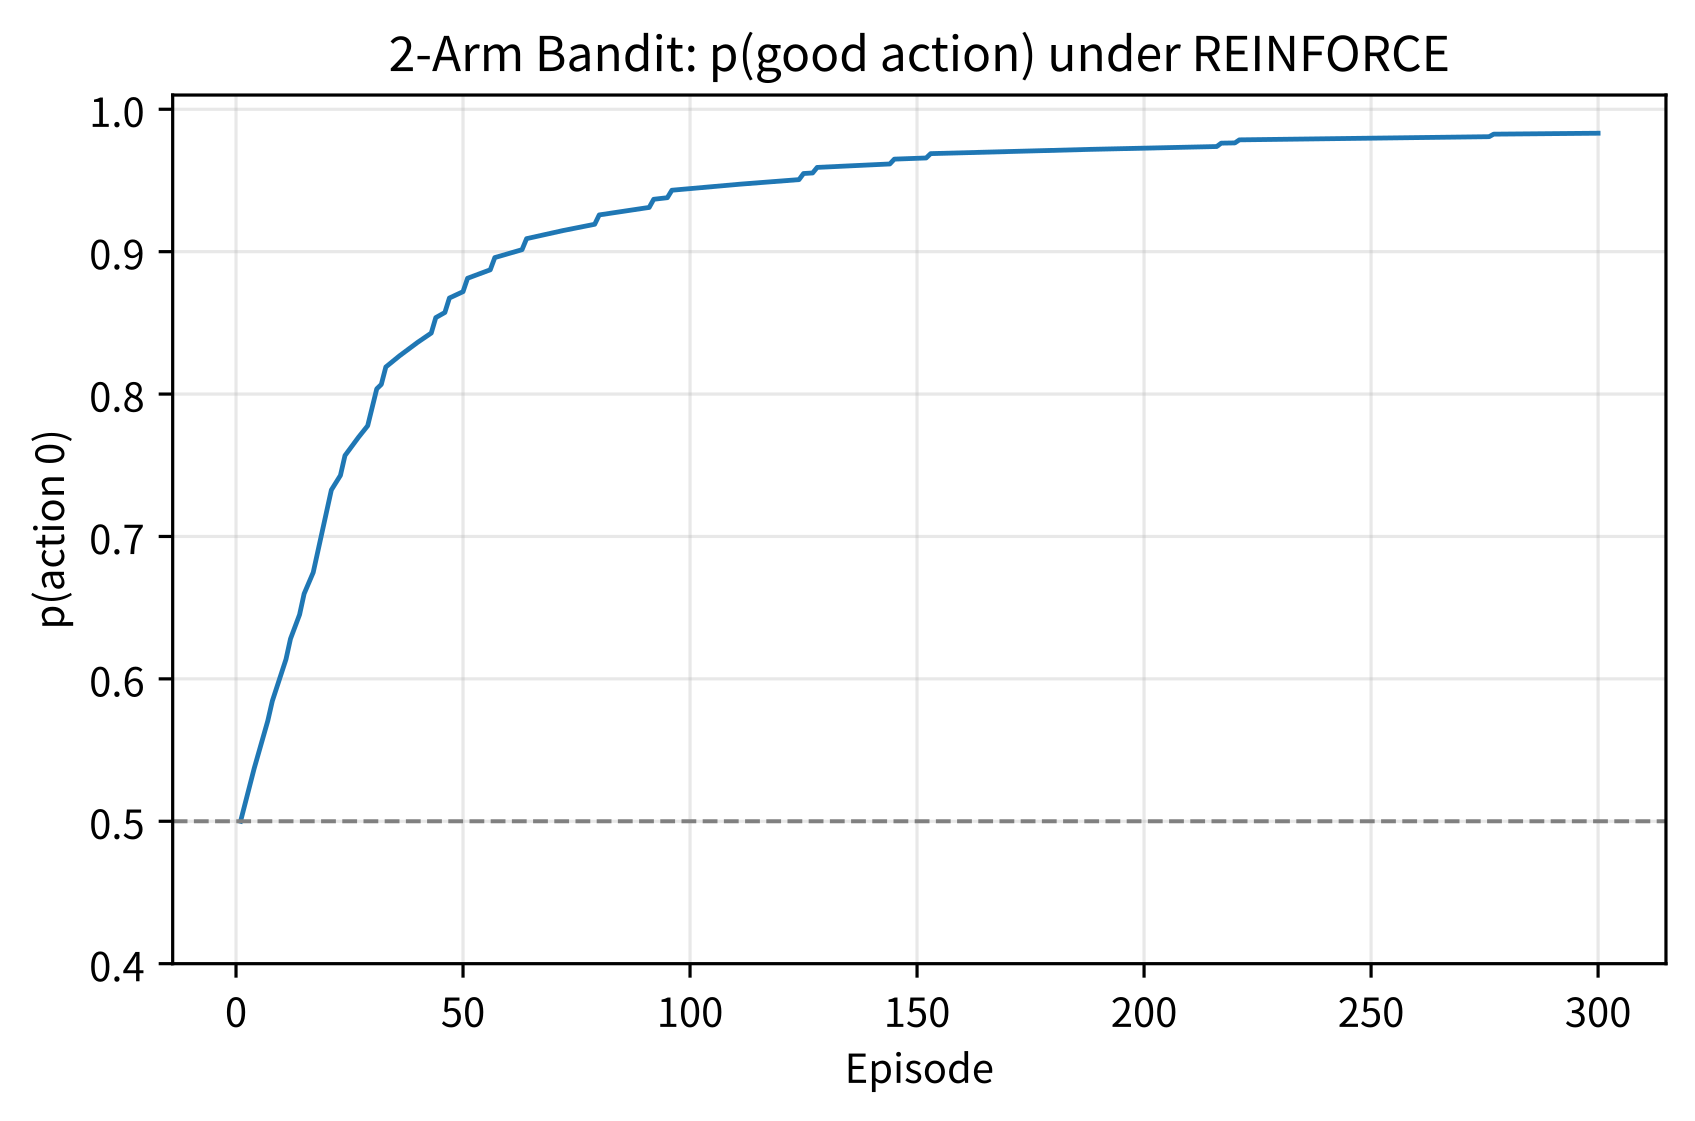
\includegraphics[width=\linewidth]{ch10_2_reinforce_bandit.png}
      \vskip0.3em
      {\footnotesize $p$(행동 0): 0.5 (무작위) $\to$
      0.98 (거의 확정), 300 에피소드.}
    \end{column}
  \end{columns}
  \vskip0.3em
  \kq{곡선의 ``모양'': 학습의 대부분(0.5$\to$0.87)은 \textbf{처음
  50 에피소드}에 집중, 이후 1에 점근하듯 느림.}
\end{frame}

\begin{frame}{왜 이렇게 느리게 수렴하는가}
  \begin{block}{힌트}
    $p_0$ 가 1에 가까워질수록:
    \begin{itemize}
      \item 그래디언트 성분 $(1-p_0)$ 이 \textbf{줄어}
        ``더 올릴 힘''이 약해지고,
      \item ``나쁜 행동''을 샘플링해 자신감을 \textbf{교정}해줄
        기회도 줄어듦.
    \end{itemize}
    $\to$ 단일 샘플 $G_t$ 로 업데이트하는 \textbf{모든} REINFORCE
    계열 알고리즘의 \textbf{본질적 특성}.
  \end{block}
  \vskip0.4em
  {\footnotesize 10.3절에서 가치함수로 추정하는 것(또는 더 많은
  샘플을 쓰는 것)이 이 ``느림''을 공격하는 방법 중 하나.}
  \vskip0.6em
  \begin{block}{왜 이게 model-free인가 --- 다시 한 번}
    궤적 확률 $P(\tau;\theta) = \prod_t \pi_\theta(a_t|s_t)\,
    P(s_{t+1}|s_t,a_t)$ 를 \textbf{로그}로 바꾸면, 환경 전이확률 항은
    $\theta$ 와 \textbf{무관}해서 미분하면 \textbf{사라짐}.
    최종 식에는 정책 $\pi_\theta$ \textbf{만} 남고 환경 모델은
    전혀 등장하지 않음 --- model-free의 핵심 성질이 여기서 나옴.
  \end{block}
\end{frame}

\begin{frame}[fragile]{PyTorch REINFORCE (1/2): PolicyNet과 에피소드 실행}
  자동 미분을 이용하면 훨씬 \textbf{간결}하게 같은 알고리즘:
\begin{lstlisting}
import torch, torch.nn as nn

class PolicyNet(nn.Module):
    def __init__(self, state_dim, n_actions):
        super().__init__()
        self.net = nn.Sequential(
            nn.Linear(state_dim, 64), nn.ReLU(),
            nn.Linear(64, n_actions))
    def forward(self, x):
        return torch.softmax(self.net(x), dim=-1)

policy = PolicyNet(4, 2)              # CartPole: 상태 4차원, 행동 2개
opt  = torch.optim.Adam(policy.parameters(), lr=1e-2)

def run_episode(env, seed):
    s, _ = env.reset(seed=seed)
    log_probs, rewards = [], []
    for _ in range(500):
        probs = policy(torch.tensor(s, dtype=torch.float32))
        dist  = torch.distributions.Categorical(probs)
        a = dist.sample()
        log_probs.append(dist.log_prob(a))    # log pi_theta(a|s)
        s, r, term, trunc, _ = env.step(a.item())
        rewards.append(r)
        if term or trunc: break
    return log_probs, rewards
\end{lstlisting}
\end{frame}

\begin{frame}[fragile]{PyTorch REINFORCE (2/2): 리턴 계산과 업데이트}
\begin{lstlisting}
def reinforce_update(log_probs, rewards, gamma):
    G, returns = 0.0, []
    for r in reversed(rewards):            # 루프 1: 리턴 역산
        G = r + gamma * G
        returns.insert(0, G)
    returns = torch.tensor(returns, dtype=torch.float32)
    returns = (returns - returns.mean())   # 분산 감소용 정규화
            /  (returns.std() + 1e-8)
    loss = -sum(lp * g for lp, g in zip(log_probs, returns))
    # 경사 "상승"이므로 부호 반전 (최소화 프레임워크에서 +로)
    opt.zero_grad(); loss.backward(); opt.step()
\end{lstlisting}
  \vskip0.4em
  \begin{block}{$\log\pi_\theta$ 를 손으로 미분하지 않아도 됨}
    \texttt{torch.distributions.Categorical} 이
    \texttt{log\_prob()} 제공 $\to$ 10.1절의 $\log\pi_\theta(a_t|s_t)$
    를 \textbf{그대로} 획득. 손실을 $-\texttt{log\_prob} \times G$
    로 정의하고 \texttt{.backward()} 호출 $\to$ PyTorch가
    Policy Gradient Theorem의 그래디언트를 \textbf{자동} 계산
    (one-vs-rest 식이 정확히 내부 계산 값).
  \end{block}
\end{frame}

\begin{frame}{CartPole 300 에피소드: ``100대에 포화되지 못한다''}
  \begin{columns}[T]
    \begin{column}{0.52\textwidth}
      \scriptsize
      \begin{verbatim}
처음 20 에피소드 평균 리턴:  14.05
마지막 20 에피소드 평균 리턴: 99.45
학습 중 도달한 최고 리턴:    500.0
      \end{verbatim}
      \small
      \begin{itemize}
        \item seed 0 기준(실제 검증, 실습 노트북에서 재현).
        \item 정확한 숫자는 시드에 따라 다름
          (다른 seed: 마지막 20 평균 144$\sim$191,
          최고 359$\sim$500).
      \end{itemize}
    \end{column}
    \begin{column}{0.48\textwidth}
      \centering
      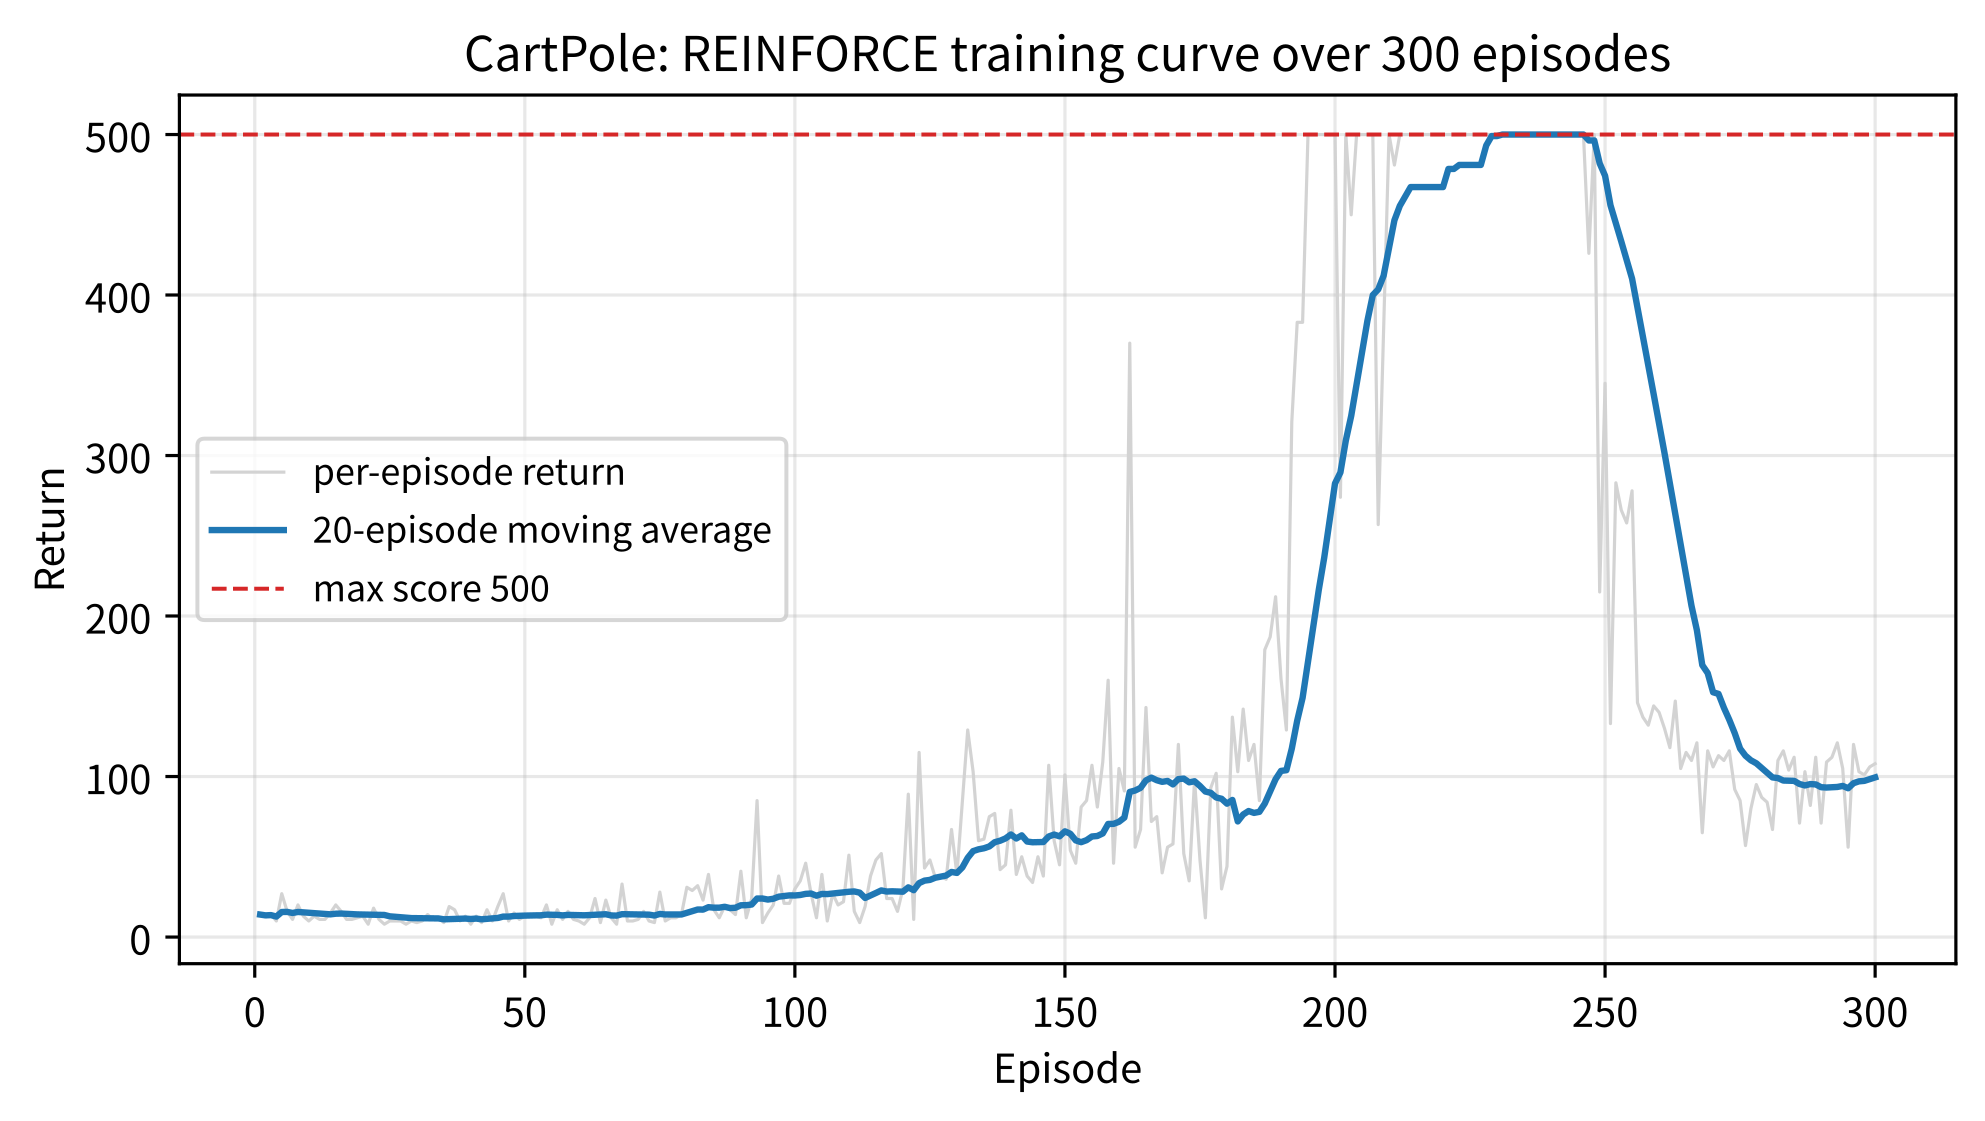
\includegraphics[width=\linewidth]{ch10_2_reinforce_cartpole_curve.png}
      \vskip0.3em
      {\footnotesize 연회색 = 에피소드별 리턴, 파란 실선 =
      20 에피소드 이동평균(약 13 $\to$ 약 100), 빨간 점선 =
      만점 500. 개별 에피소드는 큰 변동(노이즈).}
    \end{column}
  \end{columns}
  \vskip0.4em
  \kq{큰 그림은 안정적: ``10대에서 100대로 오르지만 500에
  도달해 \textbf{포화되지 못한다}.''}
\end{frame}

\begin{frame}{DQN(Ch.\,9.3)과 비교: 느리고 불안정하게}
  \small
  \begin{tabular}{@{}lccc@{}}
    \toprule
     & 처음 20 회 평균 & 마지막 20 회 평균 & 최고 \\
    \midrule
    REINFORCE (Ch.\,10.2) & 14.05 & 99.45 & 500 \\
    DQN (Ch.\,9.3, 같은 300 에피소드) & -- & 145.35 & 500 \\
    \bottomrule
  \end{tabular}
  \normalsize
  \vskip0.5em
  \begin{itemize}
    \item REINFORCE는 개선되긴 했으나 (14.05 $\to$ 99.45),
      DQN보다 \textbf{훨씬 느리고 불안정하게} 학습.
    \item 이건 REINFORCE 구현이 \textbf{잘못된 게 아니라},
      10.3절의 \textbf{``REINFORCE는 분산이 크다''는 알려진
      한계}가 실제 숫자로 드러난 것.
  \end{itemize}
  \vskip0.3em
  \begin{block}{다음}
    10.3 Actor-Critic, Ch.\,11 PPO가 정확히 \textbf{이 문제}를
    개선하려는 시도.
  \end{block}
\end{frame}

\begin{frame}{자주 하는 실수: 리턴을 정규화하지 않고 그대로 쓰기}
  \begin{itemize}
    \item \texttt{returns = (returns - returns.mean()) /
      (returns.std() + 1e-8)} 줄을 \textbf{빼고} 원래 $G_t$ 를
      그대로 쓰면?
    \item CartPole의 리턴은 \textbf{항상 양수}(매 스텝 $+1$) $\to$
      모든 행동의 그래디언트가 \textbf{항상} ``그 행동의 확률을
      높이는'' 방향으로만 움직임.
    \item 나빴던 행동조차 ``\textbf{덜 좋았을 뿐} 여전히 양수''라서
      그 확률을 계속 높이려 듦.
  \end{itemize}
  \vskip0.4em
  \begin{block}{해결: 평균을 빼면 방향이 생기게 됨}
    ``베이스라인을 빼서 어떤 행동이 평균보다 \textbf{나았는지/
    나빴는지}를 상대적으로 비교'' (10.3 아이디어)를 가장
    단순하게 구현한 것이 바로 이 정규화 ---
    평균보다 나빴던 행동은 \textbf{음수 신호}를 받아 확률이
    실제로 \textbf{낮아짐}.
  \end{block}
\end{frame}

\begin{frame}{``평균을 빼도'' 그래디언트 기댓값이 안 바뀌는 이유}
  상태 $s_t$ 에만 의존(행동과 무관)한 값 $b(s_t)$ 를 빼도,
  그래디언트 기댓값은 \textbf{그대로}:
  \[
  \mathbb{E}_{a\sim\pi}\Big[ (G_t - b(s_t))\, \nabla_\theta\log\pi_\theta(a|s_t) \Big]
  = \mathbb{E}_{a\sim\pi}\big[ G_t \nabla_\theta\log\pi \big]
  - b(s_t)\, \underbrace{\mathbb{E}_{a\sim\pi}
  \big[ \nabla_\theta \log\pi_\theta(a|s_t) \big]}_{=\, \nabla_\theta
  \sum_a \pi_\theta(a|s_t) = \nabla_\theta 1 = 0}
  \]
  \begin{itemize}
    \item 핵심은 \textbf{밑줄 친 부분}: ``각 행동의 확률합이 항상
      1''이므로 확률가중평균 그래디언트는 0.
    \item \kq{\kb{베이스라인은 행동을 의존하면 안 된다}} ---
      $b$ 가 $a$ 에도 의존하면 이 소거가 깨져 기댓값이 실제로
      바뀜(편향).
    \item 위 정규화 줄 = 이 형태의 가장 단순한 베이스라인 ---
      ``\textbf{에피소드당 평균 리턴}을 빼기''.
  \end{itemize}
\end{frame}

\begin{frame}{솔직한 비고: 정규화 효과가 시드에 따라 갈릴 수 있다}
  같은 CartPole에서 정규화 줄을 빼고 재검증한 결과
  (마지막 20 에피소드 평균):
  \small
  \begin{tabular}{@{}lccc@{}}
    \toprule
     & seed 0 & seed 1 & seed 2 \\
    \midrule
    정규화 \textbf{있음} (베이스라인) & 99.45 & 191.10 & 144.20 \\
    정규화 \textbf{없음} ($G_t$ 그대로) & 383.10 & 139.00 & 76.15 \\
    \bottomrule
  \end{tabular}
  \normalsize
  \vskip0.5em
  \begin{itemize}
    \item seed 0에서는 오히려 ``정규화 안 한 쪽''이 더 잘했고,
      seed \textbf{사이의 편차도 넓음}.
  \end{itemize}
  \begin{block}{``정규화가 무의미하다''는 뜻이 \textbf{아니라}}
    \textbf{300 에피소드라는 데이터량으로는 베이스라인의 이득
    (분산 감소)이 노이즈에 묻힐 수 있다}는 뜻.
    베이스라인의 주된 효과는 ``더 빠르게''가 아니라
    \textbf{``에피소드 노이즈 한 방에 학습 곡선을 주행하지
    않게''} 하는 것 --- 에피소드가 많고 리턴 편차가 클수록
    이득이 뚜렷해짐.
  \end{block}
  {\footnotesize 베이스라인의 ``적은'' 형태(에피소드당 평균이
  아니라 \textbf{상태별} 가치함수 $V(s_t)$)가 10.3절의
  Actor-Critic.}
\end{frame}

\begin{frame}{역사: 40년 전부터 있는 이름}
  \begin{itemize}
    \item ``좋은 궤적의 행동 확률을 올리고, 나쁜 궤적의 행동
      확률을 내린다''는 아이디어는 생각보다 \textbf{오래됨}.
    \item Sutton의 \textbf{1984년} MIT 박사 학위논문에는 이미
      ``행동의 결과를 보면서 행동 확률을 조정''하는 같은 계열
      알고리즘.
    \item \textbf{REINFORCE} (REINforce = reinforcement + force
      줄임)라는 구체적 알고리즘은 \textbf{1990년대에} 정식 제안.
    \item Williams (1992): 이 갱신 규칙이 통계학의 고전 기법인
      \kb{스코어함수 추정치}와 \textbf{정확히 같은 식}임을 보임
      (확률적 최적화 문헌에서는 \kb{likelihood ratio method}로
      동일 알고리즘이 나타남).
  \end{itemize}
  \vskip0.3em
  {\footnotesize ``고전 통계의 미분 추정 기법을 강화학습에 적용한
  것''으로 읽을 수도 있음 --- 10.1 역사와 같은 뿌리.}
\end{frame}

\begin{frame}{REINFORCE는 30년째 안 바뀐 ``참고 기준''}
  \begin{itemize}
    \item REINFORCE가 30년째 \textbf{바뀌지 않는}
      \textbf{reference algorithm}.
    \item 갱신 식 $\theta \leftarrow \theta + \alpha\, G_t\,
      \nabla\log\pi_\theta(a_t|s_t)$ 는, 아래 두 가지를 고를 때만
      예외로, \textbf{오늘날 모든 정책 그래디언트 알고리즘에서
      같은 식}:
    \begin{itemize}
      \item \kb{베이스라인 선택} (10.3 Actor-Critic)
      \item \kb{에피소드 경험의 재사용 횟수} (Ch.\,11 PPO)
    \end{itemize}
  \end{itemize}
  \vskip0.4em
  \begin{block}{중요한 포인트}
    이번 절이 ``\textbf{빨라서}'' 중요한 게 아니라, 이후 모든
    개선이 ``\textbf{REINFORCE의 이 특정 부분을 바꾼 것}''이라는
    사실의 \textbf{기준점}이 되어서 중요.
  \end{block}
\end{frame}

\begin{frame}{자주 묻는 질문 (10.2)}
  \small
  \begin{itemize}
    \item \kb{Q: 에피소드가 끝날 때까지 갱신 안 한다는 건
      Ch.\,5 ``몬테카를로'' 방식인가?}
      \textbf{네.} 실제 관찰된 $G_t$ 를 쓰는 점에서 MC와 같은
      구조. 다만 분류는 \textbf{네 가지 속성}으로: REINFORCE는
      \textbf{on-policy, model-free, MC 기반, 정책기반}.
      ``정책기반''이 포함된 이유: 배우는 대상이 가치표가 아니라
      \textbf{정책의 파라미터}, 갱신 방식이 ``평균''
      ($Q \leftarrow Q + \alpha(G-Q)$)이 아니라 ``경사 상승''
      ($\theta \leftarrow \theta + \alpha G \nabla\log\pi$).
      정책기반 + \textbf{TD} = 10.3 Actor-Critic ---
      ``배우는 대상(정책 vs 가치)''과 ``갱신 원리(경사 상승 vs
      부트스트랩)''은 \textbf{독립적인 축}.
    \item \kb{Q: 최고 리턴 500이 나왔는데, 마지막 20 에피소드
      평균이 왜 100 정도?}
      ``최고''는 \textbf{단일 행운 에피소드}의 기록 --- 분산이
      커서 정책이 좋아진 뒤에도 가끔 짧은 에피소드가 나오는
      것은 정상. 정책의 ``진짜'' 수준은 마지막 $N$ 에피소드의
      \textbf{평균}(또는 별도 평가 롤아웃)으로 판단 (Ch.\,6.3의
      ``탐욕적 평가로 판단'' 교훈과 같음).
    \item \kb{Q: 긴 지평선 태스크에서는 너무 느럽지 않나요?}
      \textbf{그렇다.} 에피소드 하나를 끝까지 기다리는 것은 느리고,
      $G_t$ 는 ``여기부터 끝까지'' 보상 전체를 담고 있어 분산 큼.
      10.3 Actor-Critic은 $G_t$ 를 \textbf{가치함수 기반 부트스트랩
      추정}($G_t - V(s_t)$, 어드밴티지)으로 바꿔 \textbf{매 스텝}
      갱신 $\to$ 기다림도 줄고 분산도 줄어듦.
  \end{itemize}
  \normalsize
\end{frame}

\begin{frame}{10.2 마무리: REINFORCE가 주는 가치는 ``명확함''}
  \begin{block}{한 줄 요약}
    REINFORCE는 Policy Gradient Theorem의 \textbf{가장 단순하고
    직접적인 구현} --- ``결과가 좋았던 궤적에서 고른 행동의
    확률을 올리고, 나빴던 행동의 확률은 내린다''는 것을,
    관찰된 리턴 $G_t$ 가 좋은/나쁜의 기준으로 삼아 구현.
  \end{block}
  \vskip0.4em
  \begin{itemize}
    \item 가치는 \textbf{속도가 아니라 \textbf{명확함}} ---
      코드 한 줄이 정리 한 항과 직접 대응.
    \item 이후 Actor-Critic(10.3) $\cdot$ PPO(Ch.\,11)의
      \textbf{모든 개선}은 ``REINFORCE의 이 특정 부분을 바꾼
      것'':
  \end{itemize}
  \vskip0.2em
  \small
  \begin{tabular}{@{}lll@{}}
    \toprule
     & REINFORCE (10.2) & 개선 (10.3, Ch.\,11) \\
    \midrule
    리턴 & $G_t$ 그대로 & 베이스라인 붙인 추정 ($G_t - V(s_t)$) \\
    경험 재사용 & 에피소드당 1회 & 여러 회 사용 + 클리핑 (PPO) \\
    \bottomrule
  \end{tabular}
  \normalsize
\end{frame}

% ================= SESSION 10.3 =================
\section{10.3 Actor-Critic}

\begin{frame}{Actor-Critic: 분산을 줄이는 개선}
  \begin{itemize}
    \item REINFORCE: $G_t$ (실제 관찰된 누적 보상)를 \textbf{그대로}
      사용 --- 하나의 에피소드를 샘플링한 결과라 \textbf{노이즈가
      크다}(분산 높음).
    \item \kb{Actor-Critic}: $G_t$ 대신 Ch.\,4$\cdot$6의 \textbf{가치함수}
      (Critic)로 추정한 기준값을 빼서 분산 감소 ---
      $G_t - V(s_t)$ 의 차이를 \kb{어드밴티지(advantage)}라 부름.
    \item \textbf{정책(Actor)}과 \textbf{가치함수(Critic)}를
      \textbf{동시에} 학습.
  \end{itemize}
  \vskip0.4em
  \begin{block}{핵심 아이디어 (한 줄)}
    ``정책 하나만 학습하는 것보다, \textbf{가치함수의 도움}을 받으면
    \textbf{더 안정적으로} 학습된다.''
    이 어드밴티지는 Ch.\,11의 PPO에서 \textbf{그대로 재사용}됨.
  \end{block}
  {\footnotesize Q-learning이 ``얼마나 좋은지 평가한 뒤 최선을
  고른다''는 \textbf{간접적} 전략이라면, 정책기반 방법은
  ``무엇을 할지'' \textbf{자체}를 직접, 연속 행동 공간에서도
  학습. 유한 MDP라면 최적 정책 $\pi^{*}$ 는 항상 존재 (Ch.\,4) ---
  policy gradient는 그 목표를 향해 \textbf{직접} 나아가는 방법.}
\end{frame}

\begin{frame}{먼저 문제부터: REINFORCE 신호가 ``너무 시끄러운'' 이유}
  \begin{itemize}
    \item 10.2의 CartPole REINFORCE: 처음 20 에피소드 평균 14.1
      $\to$ 마지막 20 에피소드 평균 99.5, 최고 500 --- 배운 것은
      배운 것.
    \item 그런데 \textbf{시드를 세 번} 바꿔 실행하면 학습 곡선이
      시드마다 \textbf{다른 모양}으로 나옴 --- 어떤 시드는
      98 에피소드만에 리턴 250 돌파, 다른 시드는 300 에피소드 다
      배워도 \textbf{150 안팎}.
    \item 이 ``거친'' 움직임은 코드 버그가 아니라
      \kb{REINFORCE 자체의 높은 분산}.
  \end{itemize}
  \vskip0.4em
  \begin{block}{왜 분산이 큰가}
    $G_t$ 는 ``폴이 \textbf{몇 스텝 뒤에 무너졌는가}''에 거의
    전적으로 의존 (매 스텝 $+1$). 그런데 몇 스텝 뒤로 무너지는가는
    ``이 스텝의 행동이 좋았는가''와 \textbf{별개인 요소}
    (초기 기울기의 작은 차이, 샘플링의 운).
    REINFORCE는 그 \textbf{운을 신호 크기로 그대로} 받아들임:
    운 좋게 오래 버틴 에피소드에선 그 날 행동 \textbf{전부}를 크게
    강화, 일찍 무너진 에피소드에선 전부 크게 낮춤 ---
    \textbf{노이즈 섞인 채} 경사 상승.
  \end{block}
\end{frame}

\begin{frame}{``샘플을 더 뽑아 평균''이 바로 먹지 않는 이유}
  \begin{itemize}
    \item 이 문제는 Ch.\,5 \kb{중요도 샘플링}과 \textbf{같은 뿌리}
      --- ``기댓값을 샘플 하나로 추정하면 흔들린다''.
    \item 그때의 해법 = ``\textbf{샘플을 더 뽑아 평균}''.
  \end{itemize}
  \vskip0.4em
  \begin{itemize}
    \item RL에서는 그 해법이 \textbf{그대로 먹지 않음}:
      한 에피소드의 샘플은 \textbf{현재 정책이 실제로 행동한
      결과} 자체라서, ``같은 상황에서 더 뽑자''는 말이 쉽게
      안 됨 (매 에피소드가 \textbf{새 행동의 대가}라는 비용이
      있음).
  \end{itemize}
  \vskip0.4em
  \begin{block}{Actor-Critic은 다른 길로 간다}
    샘플 하나하나에 \textbf{``기준값''}을 대고,
    \textbf{절대} 보상이 아니라 \textbf{``평균보다 얼마나 더
    좋았는지''라는 상대적 향상}으로 신호를 만든다.
  \end{block}
\end{frame}

\begin{frame}{베이스라인의 핵심 수학적 사실: 3단계로}
  $b(s_t)$ 를 \textbf{현재 상태 $s_t$ 에만 의존하고, 행동 $a_t$ 에는
  전혀 의존하지 않는} 어떤 값이라 하자 (Ch.\,4의 가치함수
  $V(s_t)$ 가 대표 예):
  \[
  \mathbb{E}_{a_t \sim \pi(\cdot|s_t)}
  \big[ \nabla_\theta \log\pi_\theta(a_t|s_t)\, b(s_t) \big]
  = b(s_t)\, \mathbb{E}_{a_t}
  \big[ \nabla_\theta \log\pi_\theta(a_t|s_t) \big]
  = b(s_t)\, \underbrace{\sum_{a_t} \nabla_\theta \pi_\theta(a_t|s_t)}_{=0}
  = 0
  \]
  세 단계:
  \begin{enumerate}
    \item $b(s_t)$ 는 $a_t$ 와 무관한 \textbf{상수}라 기댓값
      \textbf{밖으로} 나옴.
    \item $\nabla\log\pi = \nabla\pi/\pi$ 이므로
      $\sum_a \pi(a)\nabla\log\pi(a) = \sum_a \nabla\pi(a)$.
    \item 모든 행동의 확률 합은 $1$이고, \textbf{상수의 미분은 0}.
  \end{enumerate}
  \vskip0.3em
  \begin{block}{한 줄 결론}
    \[
    \mathbb{E}\big[ (G_t - b(s_t))\,\nabla_\theta\log\pi_\theta(a_t|s_t) \big]
    = \mathbb{E}\big[ G_t\,\nabla_\theta\log\pi_\theta(a_t|s_t) \big]
    - \underbrace{b(s_t)\,\mathbb{E}
    \big[ \nabla_\theta \log\pi_\theta(a_t|s_t) \big]}_{=0}
    \]
    \textbf{그래디언트 기댓값(= 진짜 기울기 방향)은 $b(s_t)$ 를
    빼도 그대로} --- 그런데 \textbf{분산만} 줄어듦
    ($G_t$ 가 크게 흔들리던 신호가 ``기준에서 얼마나 벗어나는가''로
    감소).
  \end{block}
\end{frame}

\begin{frame}{숫자로 검증: 2행동 밴딧 한 스텝}
  \begin{itemize}
    \item \textbf{1스텝 밴딧}: 행동 0 $\to$ $+1.0$, 행동 1 $\to$
      $+1.8$. $s=1$, $\pi(a|s) = \text{softmax}([0,0])$ $\to$
      $p(a=0)=p(a=1)=0.5$.
    \item \textbf{참값}: $V(s) = 0.5\times1.0 + 0.5\times1.8
      = \mathbf{1.4}$.
    \item 그래디언트: $\nabla\log\pi(a{=}0) = [0.5, -0.5]$,
      $\nabla\log\pi(a{=}1) = [-0.5, 0.5]$.
  \end{itemize}
  \vskip0.3em
  \scriptsize
  \begin{tabular}{@{}llll@{}}
    \toprule
     & $a{=}0$ 샘플 & $a{=}1$ 샘플 & 기댓값 (참 기울기) \\
    \midrule
    REINFORCE: $G_t\nabla\log\pi$
      & $+1.0\,[0.5,-0.5] = [0.5,-0.5]$
      & $+1.8\,[-0.5,0.5] = [-0.9,0.9]$
      & $0.5[0.5,-0.5]+0.5[-0.9,0.9] = [-0.2,0.2]$ \\
    베이스라인: $(G_t{-}V)\nabla\log\pi$
      & $(1.0-1.4)[0.5,-0.5] = [-0.2,0.2]$
      & $(1.8-1.4)[-0.5,0.5] = [-0.2,0.2]$
      & $[-0.2,0.2]$ \\
    \bottomrule
  \end{tabular}
  \normalsize
  \vskip0.4em
  \begin{itemize}
    \item \textbf{기댓값은 $[-0.2,0.2]$ 로 완전히 같음} ---
      둘 다 ``행동 1(보상 $+1.8$)의 확률을 올리는 방향''.
    \item 그런데 \textbf{샘플 하나하나}는 다름: REINFORCE의 첫
      성분은 매 스텝 \textbf{1.4나 튀어다니는} 신호, 베이스라인
      버전은 \textbf{두 샘플이 정확히 같은 벡터} --- 이 작은
      예에서는 분산이 \textbf{정확히 0}.
  \end{itemize}
  {\footnotesize ``평균은 그대로, 흔들림은 줄어든다'' ---
  숫자로 보임.}
\end{frame}

\begin{frame}{베이스라인이 ``틀린 값''이어도 기댓값은 안 바뀐다}
  \begin{itemize}
    \item $b = 1.9$ (참값 1.4와 \textbf{다른} 값)로 빼면:
      샘플은 $[-0.45, 0.45]$ / $[0.05, -0.05]$ 가 되지만,
      기댓값은 \textbf{여전히} $[-0.2, 0.2]$.
  \end{itemize}
  \vskip0.5em
  \begin{block}{이 사실이 실전적으로 중요한 이유 하나}
    \textbf{Critic은 ``완벽할 때까지'' 기다릴 필요가 없다.}
    처음부터 정확하지 않아도, \textbf{대략 근사한} $V$ 만 있으면
    분산은 크게 줄고 기댓값은 안 훼손됨.
    \vskip0.2em
    $\to$ ``Critic이 \textbf{쓰이면서} 학습하고, \textbf{학습하면서}
    더 정확해진다''는 상호보완 구조가 성립하는 \textbf{근거}가
    바로 이 불변성.
  \end{block}
  \vskip0.4em
  \begin{block}{\kb{어드밴티지} $A_t := G_t - V(s_t)$}
    $V(s_t) = \mathbb{E}[G_t|s_t]$ 는 ``이 상태에서의 \textbf{평균적}
    수준'' $\to$ $A_t$ = \textbf{평균 대비 향상분}.
    $A_t > 0$: 평균보다 더 좋은 결과 $\to$ 그 행동 확률
    \textbf{올림}. $A_t < 0$: 평균보다 나쁨 $\to$ \textbf{내림}.
    (10.2의 정규화 줄 = ``에피소드 내 평균''이라는 가장 느슨한
    베이스라인. Actor-Critic은 이를 \textbf{상태별 $V(s_t)$}로
    업그레이드 --- 상태 의존적 기준값)
  \end{block}
\end{frame}

\begin{frame}[fragile]{A2C 코드 (1/2): 네트워크와 에피소드 실행}
  10.2 REINFORCE 코드에서 \textbf{딱 두 가지}를 바꿈:
  (1) $G_t$ 를 $A_t = G_t - V(s_t)$ 로,
  (2) $V(s_t)$ 를 내주는 \textbf{Critic}을 하나 더 붙임.
\begin{lstlisting}
import torch, torch.nn as nn

class ActorCriticNet(nn.Module):
    def __init__(self, state_dim, n_actions):
        super().__init__()
        self.shared = nn.Sequential(
            nn.Linear(state_dim, 64), nn.ReLU())
        self.actor_head = nn.Linear(64, n_actions)  # Actor: 확률
        self.critic_head = nn.Linear(64, 1)         # Critic: V(s)
    def forward(self, x):
        h = self.shared(x)
        return (torch.softmax(self.actor_head(h), dim=-1),
                self.critic_head(h).squeeze(-1))

net = ActorCriticNet(4, 2)          # CartPole: 상태 4, 행동 2
opt = torch.optim.Adam(net.parameters(), lr=1e-3)

def a2c_episode(env, seed, gamma):
    s, _ = env.reset(seed=seed)
    states, log_probs, rewards, nexts = [], [], [], []
    for _ in range(500):
        st = torch.tensor(s, dtype=torch.float32)
        states.append(st)
        probs, _ = net(st)
        dist = torch.distributions.Categorical(probs)
        a = dist.sample()
        log_probs.append(dist.log_prob(a))   # log pi(a_t|s_t)
        s, r, term, trunc, _ = env.step(a.item())
        rewards.append(r)
        nexts.append(torch.tensor(s, dtype=torch.float32))
        if term or trunc: break
\end{lstlisting}
\end{frame}

\begin{frame}[fragile]{A2C 코드 (2/2): 두 손실함수, 두 갱신}
\begin{lstlisting}
    # --- 1) Actor 갱신: REINFORCE에서 G_t -> A_t = G_t - V(s_t)만 바꿈 ---
    G, rets = 0.0, []
    for r in reversed(rewards):
        G = r + gamma * G
        rets.insert(0, G)
    rets = torch.tensor(rets)
    vs    = torch.stack([net(st)[1] for st in states])  # V(s_t)
    adv   = rets - vs.detach()          # A_t (상수로 취급!)
    actor_loss = -sum(lp * ad for lp, ad in zip(log_probs, adv))
    opt.zero_grad(); actor_loss.backward(); opt.step()

    # --- 2) Critic 갱신: Chapter 6의 TD(0) 값 학습 그대로 ---
    with torch.no_grad():
        vnext = torch.stack([net(ns)[1] for ns in nexts])
    critic_loss = nn.functional.mse_loss(
        vs, torch.tensor(rewards) + gamma * vnext)
    opt.zero_grad(); critic_loss.backward(); opt.step()
    return sum(rewards)
\end{lstlisting}
\end{frame}

\begin{frame}{두 손실함수의 역할: 이 학기 배운 것들의 ``재조합''}
  \begin{itemize}
    \item \kb{Actor 손실} $-\sum_t \log\pi(a_t|s_t)\, A_t$
      --- 10.2 REINFORCE 손실의 $G_t$ 자리에 $A_t$ 가 들어간 것.
      10.2의 정규화 줄이 ``에피소드 평균을 뺀 초짜 베이스라인''
      이었다면, 여기서는 \texttt{vs}라는 \textbf{학습된 네트워크}의
      출력이 그 역할.
    \item \kb{Critic 손실} $(r_t + \gamma V(s_{t+1}) - V(s_t))^2$
      --- Ch.\,6의 \textbf{TD(0) 값 학습}을 \textbf{그대로} 사용.
  \end{itemize}
  \vskip0.3em
  \begin{block}{의도된 비대칭}
    Critic은 \textbf{부트스트랩}으로 배우는(분산 작음) 학습자,
    Actor는 \textbf{에피소드 리턴}(분산 큼) 신호를 쓰는 학습자
    --- \textbf{Critic이 Actor의 노이즈를 잡아주는 구조}.
    두 출력은 앞부분 \texttt{shared} 층을 \textbf{공유}하고 마지막
    출력층만 다름.
  \end{block}
  \vskip0.3em
  \begin{itemize}
    \item \kb{A2C} 이름의 유래: \textbf{A}dvantage \textbf{A}ctor-
      \textbf{C}ritic (DeepMind, 2016) --- ``A''가 바로 오늘 배운
      \textbf{어드밴티지}. (위 코드는 에피소드당 한 번 갱신하는
      간소화 버전. 원판 A2C/A3C는 매 스텝마다 갱신)
  \end{itemize}
\end{frame}

\begin{frame}{A3C: 비동기 병렬이 붙은 원판}
  \begin{columns}[T]
    \begin{column}{0.48\textwidth}
      \begin{itemize}
        \item \kb{A3C} (Mnih et al., 2016): A2C 구조에
          \textbf{비동기} 워커 여러 개가 \textbf{병렬}로 경험을
          수집$\cdot$갱신.
        \item A2C의 ``A'' = \textbf{A}dvantage, A3C의 ``A'' =
          \textbf{A}sync (비동기) --- 겹치지만 다른 글자.
        \item Atari 57종목에서 \textbf{사람 평균}을 상회하는
          학습 곡선 --- 비동기 병렬이 분산 감소를
          \textbf{실무 속도}로 바꿔준 예.
      \end{itemize}
    \end{column}
    \begin{column}{0.52\textwidth}
      \centering
      
\includegraphics[width=\linewidth]{ref_a3c.png}
      \vskip0.3em
      {\footnotesize A3C를 포함한 여러 비동기 RL 방법들의
      Atari 게임별 학습 곡선 비교 (원 논문 Figure 3).}
    \end{column}
  \end{columns}
\end{frame}

\begin{frame}{Actor-Critic 구조도 (순환)}
  \begin{columns}[T]
    \begin{column}{0.46\textwidth}
      \centering
      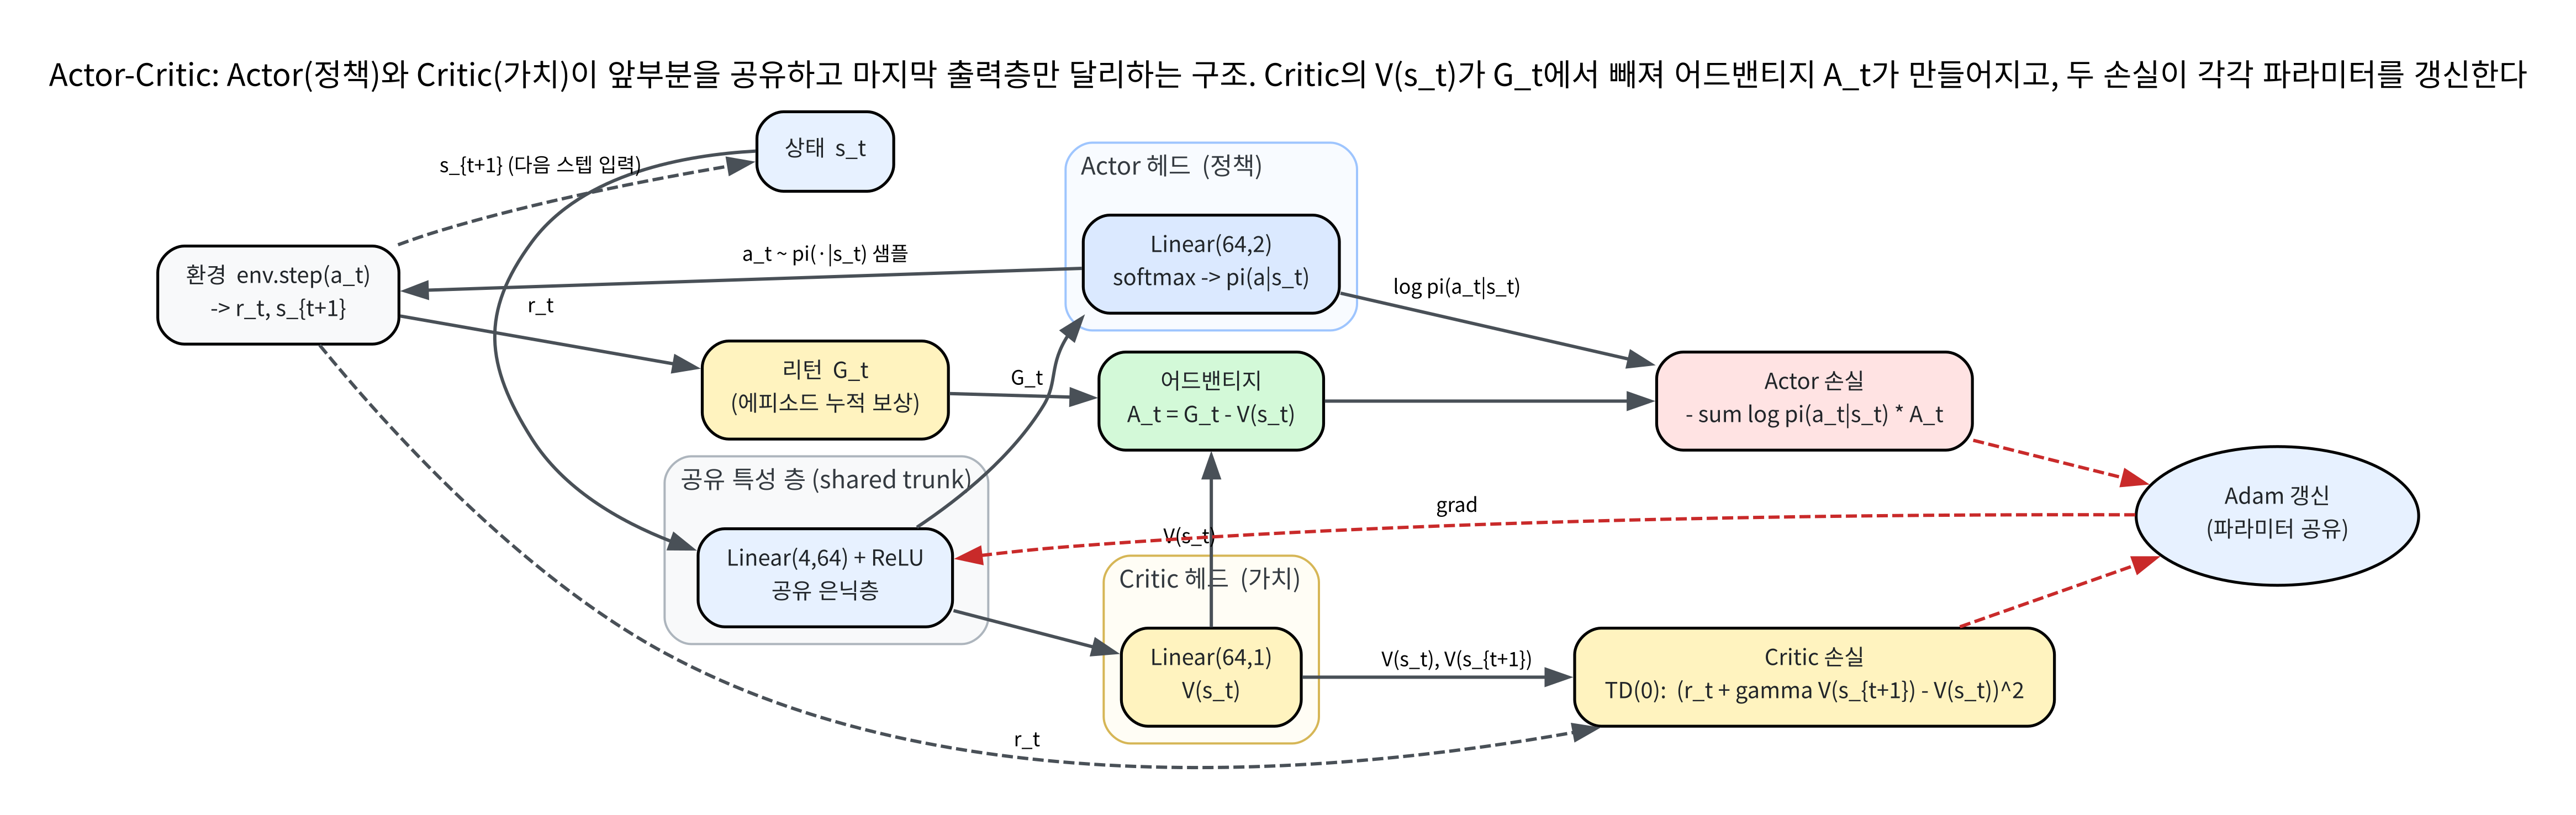
\includegraphics[width=\linewidth]{ch10_3_actor_critic_structure.png}
      \vskip0.3em
      {\footnotesize $s_t$ $\to$ 공유 특성 층 $\to$
      Actor 헤드(softmax 정책) + Critic 헤드($V(s_t)$).}
    \end{column}
    \begin{column}{0.54\textwidth}
      \begin{itemize}
        \item $s_t$ $\to$ \kb{공유 층(shared)} $\to$
          \textbf{Actor 헤드}(softmax 정책) +
          \textbf{Critic 헤드}($V(s_t)$).
        \item Actor에서 $a_t$ 샘플링 $\to$ 환경 $\to$
          $(r_t, s_{t+1})$.
        \item 에피소드 종료 후 리턴 $G_t$ 계산, $V(s_t)$ 와
          만나 \textbf{$A_t = G_t - V(s_t)$} 생성.
        \item Actor 손실 $-\sum_t \log\pi \cdot A_t$ 와 Critic
          손실(TD(0) MSE)이 각각 \textbf{Adam}으로 갱신.
        \item 갱신된 파라미터가 \textbf{공유 층으로 돌아오는
          순환} --- 매 에피소드마다 반복.
      \end{itemize}
    \end{column}
  \end{columns}
\end{frame}

\begin{frame}{실습: CartPole에서 REINFORCE vs A2C (결과)}
  두 알고리즘 \textbf{300 에피소드씩, 세 시드}(0, 1, 2):
  \small
  \begin{tabular}{@{}lcccc@{}}
    \toprule
    알고리즘 (시드) & 처음 20 평균 & 마지막 20 평균 & 최고 & 250 첫 도달 \\
    \midrule
    REINFORCE (0) & 14.1 & 99.5 & 500 & 194 \\
    REINFORCE (1) & 42.5 & 251.4 & 500 & 150 \\
    REINFORCE (2) & 17.5 & 151.9 & 500 & 98 \\
    A2C (0) & 20.6 & 211.3 & 500 & 299 \\
    A2C (1) & 21.6 & 177.9 & 500 & 277 \\
    A2C (2) & 20.4 & 184.2 & 476 & --- (미도달) \\
    \bottomrule
  \end{tabular}
  \normalsize
  \vskip0.5em
  \begin{columns}[T]
    \begin{column}{0.5\textwidth}
      \centering
      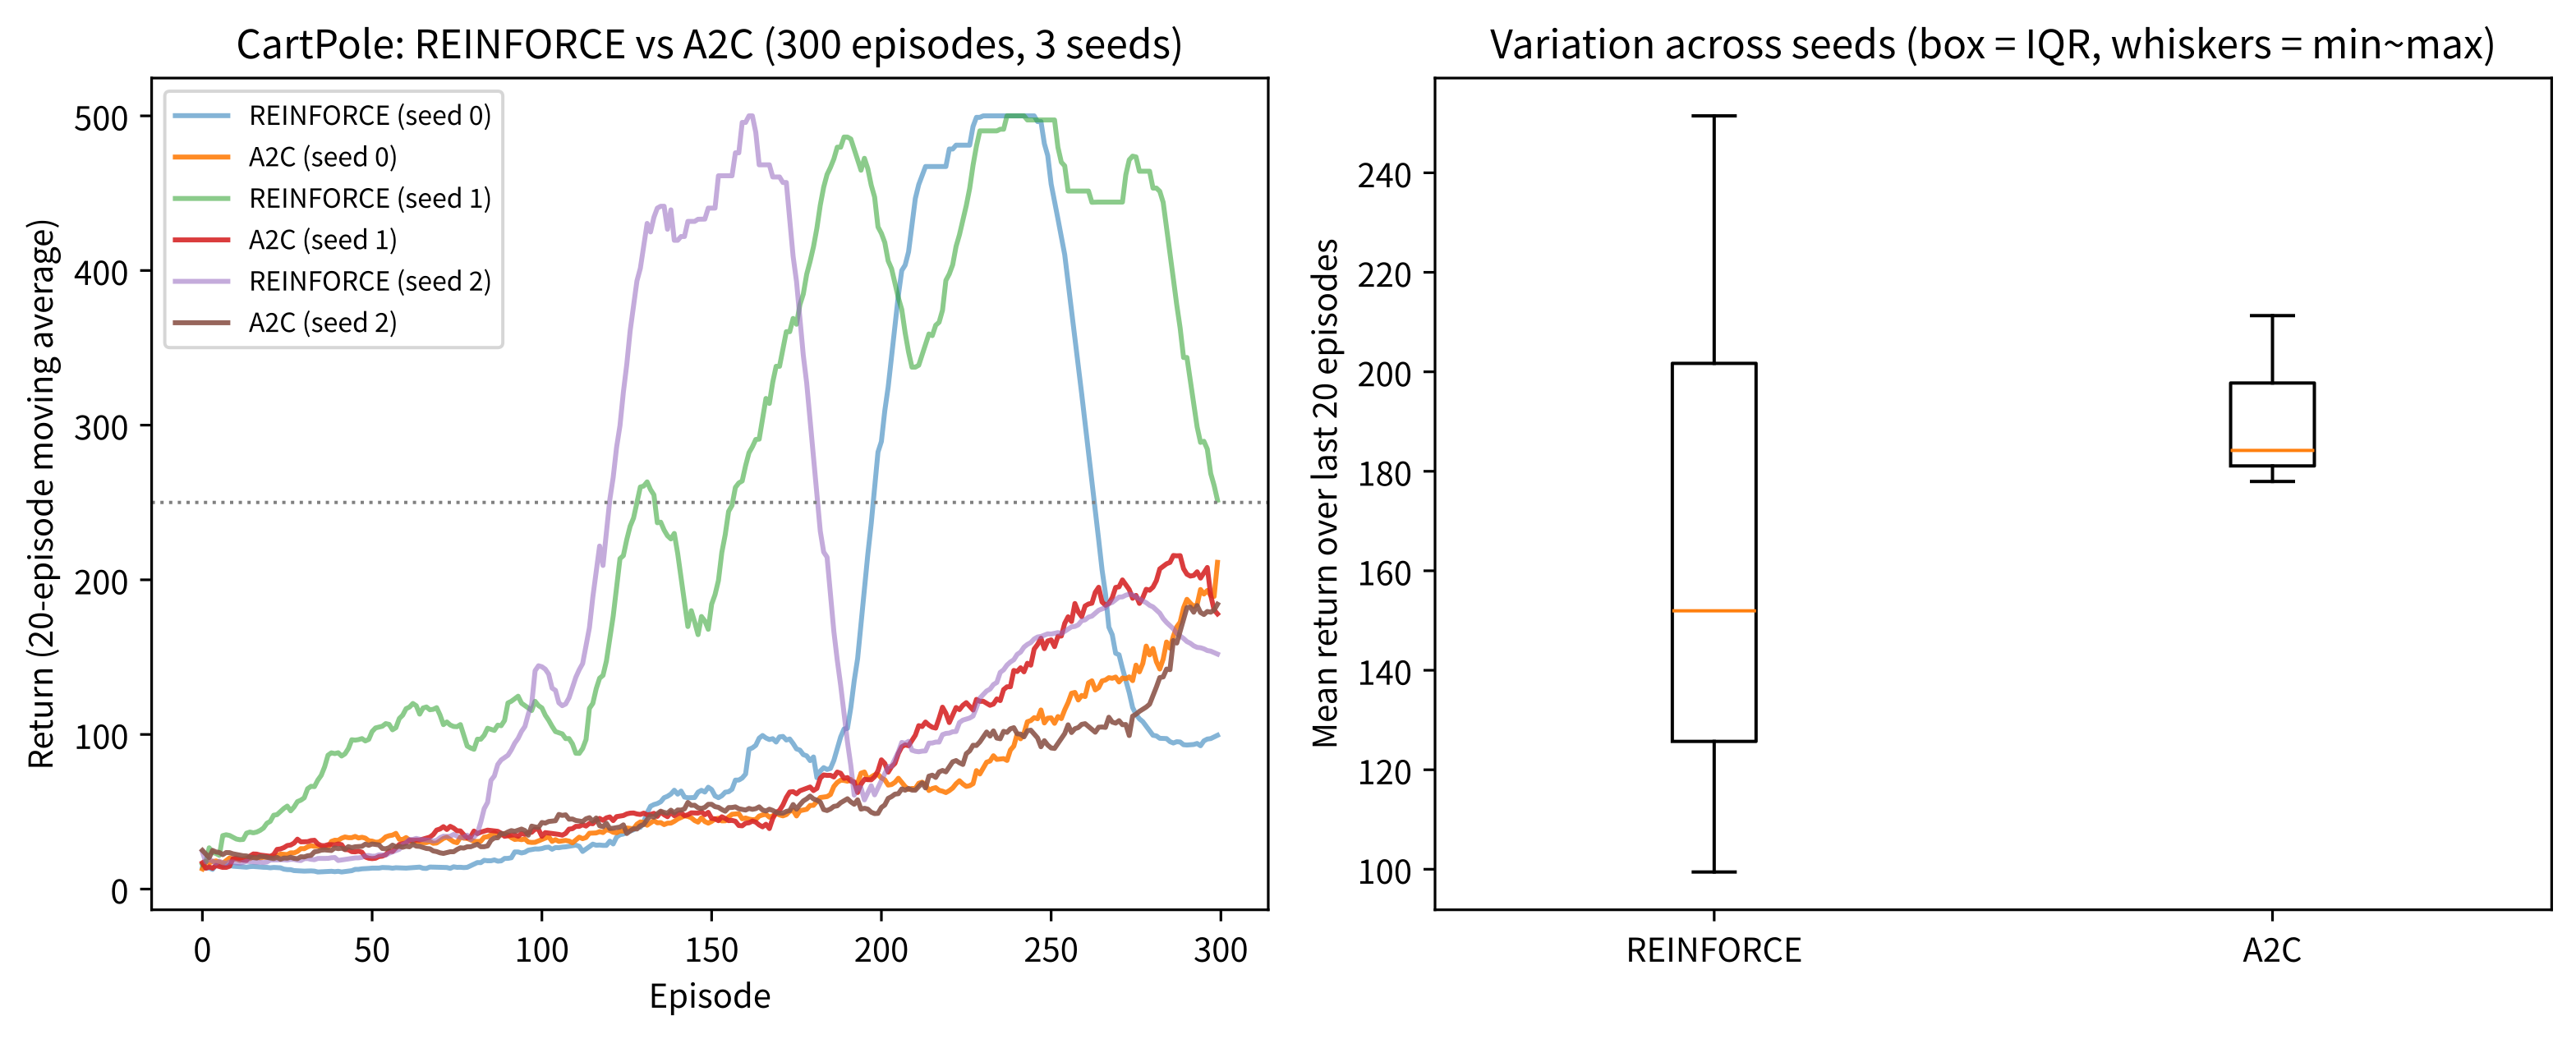
\includegraphics[width=\linewidth]{ch10_3_reinforce_vs_a2c.png}
      \vskip0.2em
      {\footnotesize 좌: 리턴 학습 곡선(20 에피소드 이동평균).
      우: 마지막 20 에피소드 평균의 시드 간 박스플롯.}
    \end{column}
    \begin{column}{0.5\textwidth}
      {\footnotesize
      REINFORCE 곡선은 시드마다 100$\sim$250 사이로
      \textbf{크게 갈라짐}. A2C 곡선은 세 시드 모두
      \textbf{180$\sim$210 대}에서 비슷한 높이로 수렴.
      박스플롯: A2C의 박스가 REINFORCE보다 \textbf{좁음}
      (시드 간 변동이 작음).}
    \end{column}
  \end{columns}
\end{frame}

\begin{frame}{세 가지로 읽기: 균일한 시작, 좁은 끝, ``속도''}
  \begin{enumerate}
    \item \kb{시작점은 A2C가 균일하다} --- 처음 20 에피소드
      평균이 REINFORCE는 $14.1\sim42.5$ 로 \textbf{흩어진}
      반면, A2C는 $20.4\sim21.6$ 로 \textbf{모임} ---
      ``시드 불운''의 영향이 기준값을 빼면서 줄었음.
    \item \kb{마지막 20 에피소드도 A2C가 좁다} --- A2C는
      $178\sim211$ 의 좁은 밴드, REINFORCE는 $99.5\sim251.4$ 로
      \textbf{150 넘게 벌어짐} --- 분산 감소가 시드 간
      \textbf{일관성}으로 나타남.
    \item \kb{도달 ``속도''는 이야기가 다름} --- 이 실험(300
      에피소드, 시드 0$\sim$2)에서는 REINFORCE가 오히려
      250 돌파가 빠른 시드가 \textbf{있었음}.
  \end{enumerate}
  \vskip0.3em
  \begin{block}{``REINFORCE가 더 좋다''는 뜻이 \textbf{아님}}
    분산이 크면 \textbf{위쪽으로도} 많이 튀기 때문.
    분산 감소의 실제 이득 --- \textbf{안정성을 유지하면서}
    학습을 \textbf{훨씬 오래, 훨씬 큰 환경}에서 돌릴 수 있게
    된 것 --- 은 Ch.\,11에서 PPO가 어드밴티지를 \textbf{클리핑된
    목적함수}에 재사용하면서 비로소 온전히 수확됨.
  \end{block}
\end{frame}

\begin{frame}{자주 하는 실수 1: \texttt{.detach()}를 빼는 것}
  \begin{itemize}
    \item \texttt{adv = rets - vs.detach()} --- \texttt{vs}는
      \texttt{net}의 \textbf{Critic 헤드 출력}.
    \item \texttt{.detach()}를 빼면 \texttt{actor\_loss.backward()}
      의 그래디언트가 \texttt{vs}를 타고 \textbf{Critic 헤드
      파라미터까지} 흘러가, \textbf{Actor 갱신 과정에서 Critic도
      함께} 갱신됨.
    \item ``두 손실이 각자 역할을 할 것''이라는 \textbf{구조가
      무너짐}.
  \end{itemize}
  \vskip0.4em
  \begin{block}{왜 \texttt{.detach()}가 필요한가}
    어드밴티지는 Actor 손실 안에서는 \textbf{상수}(미분 대상이
    아닌 곱수)로 취급해야 하므로.
    \vskip0.2em
    이 버그는 ``Critic이 이상하게 빨리/느리게 학습하는'' 형태로만
    나타나서 \textbf{찾기 어렵다}.
  \end{block}
\end{frame}

\begin{frame}{자주 하는 실수 2$\cdot$3: Critic에 MC 리턴, 속도 변화
  를 버그로 판단}
  \kb{2. Critic 목표값에 $G_t$(MC 리턴) 사용}
  \begin{itemize}
    \item Critic 손실을 $(G_t - V(s_t))^2$ 로 쓰면 Critic도
      \textbf{MC 학습자}가 됨 --- 안 \textbf{틀리지만},
      \textbf{부트스트랩이 사라져 Critic의 분산이 커짐}.
    \item Critic은 ``Actor의 노이즈를 \textbf{잡아줄 사람}''인데
      자기 자신이 노이즈가 많으면 기준값 $V(s_t)$ 가 \textbf{흔들리고},
      그 흔들림이 \textbf{그대로} Actor의 어드밴티지에 전이.
    \item \textbf{의도된 설계}: Critic은 \textbf{TD(0)}(Ch.\,6
      부트스트랩, 분산 작음), Actor는 \textbf{MC 리턴} ---
      이 \textbf{비대칭}.
  \end{itemize}
  \vskip0.4em
  \kb{3. ``베이스라인 넣었더니 학습 속도가 달라졌다''를 버그로
  판단}
  \begin{itemize}
    \item 베이스라인은 \textbf{기댓값}(진짜 기울기 방향)은
      \textbf{바꾸지 않}지만 \textbf{분산은} 바꿈 $\to$ 신호
      \textbf{크기}가 달라져 \textbf{실효 스텝 크기}가 달라지고,
      \textbf{학습 속도}가 바뀌는 것은 \textbf{정상}.
    \item 속도 변화 $\ne$ 기댓값(방향) 깨짐 --- 실제로는
      \textbf{변하지 않음} (앞 밴딧 예의 $b=1.9$ 행이 증거).
  \end{itemize}
\end{frame}

\begin{frame}{역사적 일화: 뇌의 도파민이 바로 TD 오차 (Schultz, Dayan,
Montague, 1997)}
  \begin{itemize}
    \item ``TD 오차''가 단순한 \textbf{수학적 편의}가 아니라는
      증거가 \textbf{1997년}에 나옴.
    \item 원숭이 뇌에서 \textbf{도파민 신경세포}가 보상을 받을
      때마다:
    \begin{itemize}
      \item \textbf{예측보다 좋으면} 발화량 \textbf{증가},
      \item \textbf{예측보다 나쁘면} \textbf{감소},
      \item \textbf{예측이 정확히 서 있으면} 보상이 오기
        \textbf{전}의 신호(큐) 시점에 발화가 \textbf{앞당겨짐}.
    \end{itemize}
  \end{itemize}
  \[
  \delta_t = r_t + \gamma V(s_{t+1}) - V(s_t)
  \quad \text{--- \textbf{정확히 TD 오차}}
  \]
  \begin{block}{의미}
    ``예측하지 못했던 좋은 소식''을 보내는 \textbf{뇌의 신호}와,
    강화학습의 ``예측 오차'' 신호가 \textbf{수학적으로 일치}.
    대응: ``Critic''(값 예측) $\leftrightarrow$ \textbf{도파민 회로},
    ``Actor''(신호를 행동 선택에) $\leftrightarrow$ \textbf{기저핵
    회로}. 강화학습 이론이 \textbf{생물학 신호를 설명}에 성공한,
    이 분야에서 가장 유명한 일화 중 하나.
    {\footnotesize (11.3절의 GAE도 이 TD 오차 $\delta_t$ 를
    \textbf{여러 개 가중평균}한 것 --- 같은 뿌리)}
  \end{block}
\end{frame}

\begin{frame}{자주 묻는 질문 (10.3)}
  \small
  \begin{itemize}
    \item \kb{Q: Actor와 Critic은 왜 따로 학습하나? 하나로
      합칠 수는 없나?}
      서로 \textbf{다른 것을 예측} --- Actor: ``어떤 행동을 할
      것인가''(정책), Critic: ``지금 상태가 얼마나 좋은가''
      (가치함수). 실제 구현은 \textbf{앞부분(특징 추출 층)을
      공유}하고 마지막 출력층만 다르게 --- 10.2
      \texttt{PolicyNet}에 가치 예측 출력 하나만 추가하면
      간단한 Actor-Critic.
    \item \kb{Q: $G_t - V(s_t)$ 를 빼도 기댓값이 그대로라는 게
      왜 참인가?}
      $V(s_t)$ 는 \textbf{행동 $a_t$ 와 무관하게 상태 $s_t$
      만으로} 결정 --- ``어떤 행동을 고르든 똑같이 빼지는
      상수''. 기댓값 관점에서 편향 없음. 샘플 하나하나로는
      $G_t$ 의 큰 변동폭이 $V(s_t)$ 만큼 \textbf{상쇄}
      $\to$ 분산은 확실히 감소.
    \item \kb{Q: on-policy인가, off-policy인가?}
      이 절의 구현은 \textbf{on-policy} --- Actor와 Critic이 모두
      \textbf{현재 정책}이 만든 경험에서만 학습, 경험 재생
      버퍼 \textbf{없음}. (off-policy Actor-Critic --- DQN +
      정책 결합, Ch.\,9 경험 재생 변형 --- 도 존재) 이번 학기
      표준 흐름 \kb{A2C $\to$ Ch.\,11 PPO}는 \textbf{on-policy}
      패밀리 안에서 ``분산을 줄이는'' 방향으로 발전.
    \item \kb{Q: 이산 공간인데 굳이 Actor-Critic? DQN이면
      됐지.}
      맞는 말에 가깝다 --- 이산이면 DQN이 더 데이터 효율적일
      때가 많음. Actor-Critic이 \textbf{필수}인 순간:
      (1) \textbf{연속 행동공간}(Ch.\,13--14 로봇)에서
      $\max_a Q(s,a)$ 를 계산할 수 없을 때,
      (2) \textbf{탐색 정책} 자체를 확률적으로 학습하고 싶을
      때. 게다가 $A_t$ 는 \textbf{PPO의 입력}이므로 PPO까지
      이 구조를 실무적으로 익숙해져 있어야 함.
  \end{itemize}
  \normalsize
\end{frame}

\begin{frame}{10.3 마무리: ``절대 보상''이 아니라 ``평균 대비
향상''}
  \begin{block}{핵심 정리}
    REINFORCE의 신호 $G_t$ 에는 \textbf{``운''}이 섞여 있다.
    \textbf{베이스라인} $b(s_t)$ --- \textbf{행동에 무관한 값} ---
    을 빼도 그래디언트의 \textbf{기댓값은 그대로}(행동의 확률
    합이 1에서), \textbf{분산만 줄어듦}.
    \vskip0.2em
    분산을 최소화하는 베이스라인은 $V(s_t)$ 자체 ---
    따라서 \textbf{가치함수를 \kb{Critic}}이라 부르고,
    $G_t - V(s_t)$ 를 \textbf{\kb{어드밴티지}}라 부르며,
    Actor는 이 어드밴티지로, Critic은 \textbf{TD(0)}으로,
    \textbf{동시에} 학습.
  \end{block}
  \vskip0.4em
  \kq{``절대 보상''이 아니라 \textbf{``평균 대비 향상''}으로
  배우는 이 한 가지 아이디어가 Ch.\,11의 PPO로 이어진다.}
\end{frame}

% ===== wrap-up =====
\begin{frame}{이번 주차 정리}
  \begin{enumerate}
    \item \kb{10.1 정리를 세웠다} --- Q를 거치지 않고 정책을
      직접 파라미터화(softmax / 조건부 정규). 로그미분 트릭이
      ``적분의 미분''과 ``단절된 샘플''이라는 벽을 \textbf{동시에}
      해산시켜 $\nabla_\theta J = \mathbb{E}_\tau[\sum_t
      \nabla_\theta\log\pi_\theta(a_t|s_t)\,G_t]$ 에 도달.
      one-vs-rest 모양과 $\mathbb{E}[\nabla\log\pi]=0$ 이
      베이스라인 논리의 씨앗.
    \item \kb{10.2 정리를 알고리즘으로} --- REINFORCE: 경사 상승 +
      단일 샘플 $G_t$ (on-policy, model-free, MC 기반, 정책기반).
      2행동 밴딧에서 ``좋은 행동 확률 $0.5 \to 0.98$'',
      CartPole 300 에피소드 $14 \to 100$. 리턴을 정규화하지
      않으면 ``덜 좋았을 뿐 양수'' 행동을 계속 올리려는 함정.
    \item \kb{10.3 거침을 고쳤다} --- 행동에 무관한 베이스라인
      $b(s_t)$ 를 빼도 \textbf{기댓값 불변, 분산만 감소}.
      최적 베이스라인 $= V^\pi(s_t)$ $\to$ \kb{Actor-Critic}:
      Actor는 어드밴티지 $G_t - V(s_t)$ 로, Critic은 TD(0)으로
      동시에 학습. A2C가 시드 간 \textbf{일관성}에서
      REINFORCE를 이김.
  \end{enumerate}
  \vskip0.6em
  \begin{block}{다음 주차 --- Chapter 11. 정책이 한 업데이트 만에
  무너지지 않게: PPO}
    이번 주에 손에 쥐게 된 두 네트워크(Actor, Critic)와 어드밴티지
    $A_t$ 가 PPO의 \textbf{재사용되는 구성 요소}. PPO는
    \textbf{클리핑}(한 업데이트의 크기를 제한) + \textbf{경험
    재사용}으로 REINFORCE의 거친 업데이트를 안정화 ---
    Ch.\,13$\sim$14 로봇 시뮬레이션(Pendulum)의 출발점.
  \end{block}
\end{frame}

\end{document}
